\section{Teoria Dei Codici}
    \subsection{Introduzione}
        Ci concentriamo adesso sul trattamento dell'informazione per poterla trasmettere.
        I messaggi che trasmettiamo possono essere codificati per vari motivi:
        \begin{itemize}
            \item {
                    Compressione:$\begin{cases}
                        \text{Lossy: con perdita dell'informazione} \nonumber\\
                        \text{Lossless: minima perdita dell'informazione} \nonumber
                    \end{cases}$\\
                    Comprimere l'informazione in eliminando ridondanza e salvando spazio di memoria e banda.
                    
                }
            \item {
                    Crittografia: per nascondere il messaggio ad utenti in ascolto sul canale che non siano il destinatario.
            }
            \item {
                    Rivelazione o correzione di errore: viene aggiunta ridondanza ad hoc per aumentare l'affidabilità del messaggio trasmesso. 
                    Si utilizzano \href{https://en.wikipedia.org/wiki/Checksum}{checksum} o \href{https://en.wikipedia.org/wiki/Reed-Solomon_error_correction}{Reed-Solomon(RS)}
            }
        \end{itemize}
        \paragraph{Capacità del canale}\label{Capacita del canale}\index{Capacità del canale}
            La capacità del canale $C$ indica la massima quantità d'informazione che può essere trasmessa in maniera affidabile su di un dato canale.
            La capacità dipende dalla banda $B$ del canale e dal rapporto segnale rumore (signal-to-noise ratio,\href{https://en.wikipedia.org/wiki/Signal-to-noise_ratio}{$SNR$}):
            \[
                C = B\log(1 + SNR)  
            \] 
        \paragraph{Canale Gaussiano}\index{Canale Gaussiano}
            Il canale Gaussiano può essere modellato come \href{https://en.wikipedia.org/wiki/Binary_symmetric_channel}{Binary Symmetric Channel (BSC)} con probabilità di errore $p$. 
            Assumiamo gli errori tra loro indipendenti ($p_{(a,b)} = p_{(a)}\dotproduct p_{(b)}$):
        \begin{figure}[H]
            \centering
            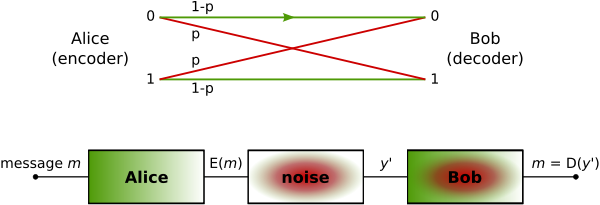
\includegraphics[width = 12cm]{media/600px-Binary_symmetric_channel_(en).svg.png}
            \label{BSC system}
            \caption{Sistema di trasmissione BSC}
        \end{figure}
        \begin{gather}
            E_{(x)}: \text{Funzione di codifica} \nonumber \\
            D_{(x)}: \text{Funzione di decodifica} \nonumber \\
            E_{(m)}: \text{Bit dell'informazione codificati} \nonumber \\
            y^\prime: E_{(m)}+ e \rightarrow \text{Informazioni con errore del canale} \nonumber \\
            m = D_{(y^\prime)}: \text{Informazione decodificata} \nonumber 
        \end{gather}
        Il canale è chiamato simmetrico perché ho la stessa probabilità errore sulla trasmissione di uno dei due bit.
        Se $X$ è il bit inviato e Y quello ricevuto allora il canale è caratterizzato dalle probabilità:
        \begin{align}
            P(Y=0|X=0) &= 1-p\nonumber \\
            P(Y=0|X=1) &= p\nonumber \\
            P(Y=1|X=0) &= p\nonumber \\
            P(Y=1|X=1) &= 1-p\nonumber 
        \end{align} 
        Assumiamo che $0\leq p \leq\frac{1}{2}$, se avessimo $p >\frac{1}{2}$ il ricevitore potrebbe scambiare l'informazione ricevuta
        (Quando riceve un $1$ lo interpreta come $0$ e viceversa) e ottenere un canale con probabilità $1-p \leq\frac{1}{2}$. 
        
        Nel corso useremo delle simbologie diverse:
        \begin{figure}[H]
            \centering
            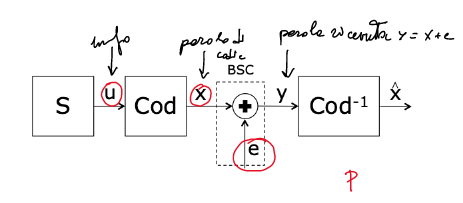
\includegraphics[width = 12cm]{media/BSC System.png}
            \label{BSC system moretti}
            \caption{Sistema di trasmissione BSC}
        \end{figure}
        \begin{gather}
            u: \text{Informazione} \nonumber \\
            x: \text{Parole di Codice} \nonumber \\
            e: \text{Errore del Canale} \nonumber \\
            y: x+e \rightarrow \text{Informazioni con errore del canale} \nonumber \\
            \overset{\wedge}{x}: \text{Informazione decodificata} \nonumber 
        \end{gather}
        \paragraph{Probabilità di errore BSC}\label{Probabilita di errore BSC}\index{Probabilità di errore BSC}
            La probabilità, per una trasmissione BSC, di sbagliare $t$ bit in una parola di $n$ bit:
            \[
                p_{(t,n)} = \binom{n}{t} p^t (1-p)^{(n-t)}
            \]
            dove il coefficiente binomiale:
            \[
                \binom{n}{t} = \frac{n!}{t!(n-t)!}
            \]
            indica tutte le possibili combinazioni di errori di $t$ bit su $n$ bit. 
        \paragraph{Tassonomia dei codici}
            \begin{itemize}
                \item {Codici lineari
                        \begin{itemize}
                            \item {
                                Codici a blocco
                                }
                            \item{
                                Codici convoluzionali
                            } 
                        \end{itemize}
                    }
                \item {
                    Definizione di un codice a blocco: 
                    \begin{figure}[H]
                        \centering 
                        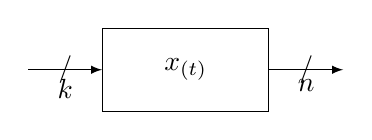
\begin{tikzpicture}[
                            node distance=2cm,
                            >=latex
                            ]

                            \node [coordinate] (input) {};
                            \node [draw, rectangle,right of = input, minimum height=3em, minimum width=6em] (block) {$x_{(t)}$};
                            \node [coordinate, right of = block] (output) {};
                            
                            \draw[draw,->] (input) -- node[midway]{$/$} node[below]{$k$} (block);
                            \draw[->] (block) -- node[midway]{$/$} node[below]{$n$} (output);
                        \end{tikzpicture}    
                    \label{Def codice a blocco}
                    \end{figure}
                    \paragraph{Rate del Codice}:\index{Rate del Codice}
                        {
                            \[
                                R = \frac{k}{n}  
                            \]
                            La condizione è che $n>k$ se non fosse così avrei perdita d'informazione, da $k$ bit passo a $n$ aggiungendo
                            ridondanza e codificando i miei dati. Possiamo quindi stimare il valore tipico di $R$
                            \[
                                R = \frac{k}{n} <1  
                            \]
                        }
                }
                \item Rivelazione di errore:\index{Rivelazione di errore}{
                    Consiste nella capacità di scoprire la presenza di errori causati dal rumore o da altri fenomeni deterioranti 
                    durante una trasmissione di dati (es. tramite il \href{https://it.wikipedia.org/wiki/Bit_di_parit%C3%A0}{bit di parità}).
                }
                \item {Correzione di errore:\index{Correzione di errore}{
                    Consiste invece nell'ulteriore abilità di ricostruire i dati originali, eliminando gli errori occorsi durante la trasmissione.
                    Vi sono due differenti schemi di base per la progettazione della codifica di canale e del protocollo per un sistema che corregge gli errori:
                    \begin{itemize}
                        \item {
                            ??\href{https://it.wikipedia.org/wiki/Automatic_repeat-request}{Automatic repeat-request} (ARQ): Il mittente invia i dati ed anche un codice a rilevazione d'errore, che sarà
                            utilizzato in ricezione per individuare gli eventuali errori, ed in tal caso chiedere la ritrasmissione dei dati
                            corrotti. In molti casi la richiesta è implicita; il destinatario invia un acknowledgement (ACK) di corretta 
                            ricezione dei dati, ed il mittente re-invia solo quei dati per i quali non ha ricevuto, entro un prefissato tempo 
                            limite (timeout), il corrispondente ACK.
                        }
                        \item{
                            ??\href{https://it.wikipedia.org/wiki/Forward_Error_Correction}{Forward Error Correction} (FEC): Il mittente codifica i dati con un codice a correzione d'errore 
                            (error correction code, ECC) ed invia il messaggio codificato. Il destinatario non invia mai alcun 
                            messaggio verso il mittente; esso decodifica ciò che riceve nella maniera più simile possibile a quella di un 
                            certo insieme prefissato di parole accettabili. Tali codici sono realizzati in modo tale che dovrebbe occorrere 
                            una quantità "irragionevole" di errori nei dati, affinché il destinatario decodifichi erroneamente, ottenendo 
                            finalmente dei dati diversi da quelli effettivamente inviatigli.
                        } 
                    \end{itemize}
                    In generale un codice a blocco che ha rate $\frac{k}{n}$ mappa $k$ bit su $n$ bit usando $2^k$ parole di codice di dimensione n
                }}
            \end{itemize}

        \subsubsection{Esempio codici a blocco: codici a ripetizione}
            É un esempio di codice a correzione d'errore: il funzionamento si basa sulla ripetizione dell'informazione più volte. Il destinatario
            si accorge di un errore di trasmissione poiché il flusso di dati ricevuto non è la ripetizione di un singolo messaggio e, inoltre, 
            il destinatario può recuperare il messaggio originale guardando il messaggio ricevuto nel flusso di dati che si verifica più spesso.

            Nel caso di un codice binario di ripetizione, esistono due parole in codice - tutte uno e tutti zeri - che hanno una lunghezza n. 
            Pertanto, la distanza minima di Hamming (\ref{Distanza di Hamming}) del codice è uguale alla sua lunghezza. Ciò conferisce al codice 
            di ripetizione, con $R = \frac{1}{n}$,una capacità di rivelazione di errori pari a $n-1$ e correzione degli errori (cioè correggerà fino agli errori in qualsiasi parola del codice) di $\frac{n-1}{2}$ per n dispari(\ref{Probabilita di errore BSC}).\\
            Esempio:\\
            \indent{$R = \frac{1}{3} \rightarrow$ ha solo 2 parole di codice:}
            \begin{align}
                u=0 \rightarrow x = [000]\nonumber \\
                u=1 \rightarrow x = [111]\nonumber
            \end{align} 
            Il ricevitore effettua una decodifica a maggioranza: decide per il bit che comprare più volte della parola ricevuta.
            \begin{align}
                y = [000] \rightarrow \overset{\wedge}{x} = [000] \rightarrow \overset{\wedge}{u} = 0 \nonumber \\
                y = [010] \rightarrow \overset{\wedge}{x} = [000] \rightarrow \overset{\wedge}{u} = 0 \nonumber \\
                y = [101] \rightarrow \overset{\wedge}{x} = [111] \rightarrow \overset{\wedge}{u} = 1 \nonumber
            \end{align}
            \paragraph{Evento errore:} l'evento errore per un codice a correzione di errore consiste nel non essere in grado di correggere
            tutti gli errori introdotti dal canale. Se la probabilità di errore sul bit $p_{e,b}$ è piccola, la probabilità di errore 
            $p_{e,W}$ per il codice può essere approssimata dal primo evento che determina la ricezione errata (nel caso dei codici a ripetizione a $R = \frac{1}{3}$ 
            si verifichino $2$ errori).
            \begin{itemize}
                \item {$R = \frac{1}{3}$
                    \begin{itemize}
                        \item {
                            Se $p_{e,b} = 0.1 \Rightarrow p_{e,W} \approx 2.7\dotproduct 10^{-2} $ 
                        }
                        \item {
                            Se $p_{e,b} = 0.01 \Rightarrow p_{e,W} \approx 2.97\dotproduct 10^{-4} $ 
                        }
                    \end{itemize}
                }
                \item {$R = \frac{1}{5}$
                    \begin{itemize}
                        \item {
                            Se $p_{e,b} = 0.1 \Rightarrow p_{e,W} \approx 8.1\dotproduct 10^{-3} $ 
                        }
                        \item {
                            Se $p_{e,b} = 0.01 \Rightarrow p_{e,W} \approx 9.8\dotproduct 10^{-6} $, Sviluppiamo i calcoli come esempio: 
                            \[
                                P_r \{\text{codice }R=\frac{1}{5}\text{ non riesce a correggere gli errori introdotti dal canale}\}:
                            \]
                            \begin{align}
                                P_r &= \sum_{t=3}^{5} \binom{5}{t}p^t (1-p)^{5-t},\hspace{0.2cm} p=10^{-2} \nonumber \\
                                P_r &\{\text{3 errori su 5}\}= \binom{5}{3}p^3 (1-p)^{5-3} = 10\dotproduct 10^{-6} (0.99)^2 = 9.8\dotproduct 10^{-6} \nonumber \\
                                P_r &\{\text{3 errori su 5}\}= \binom{5}{4}p^4 (1-p)^{5-4} = 5\dotproduct 10^{-8} (0.99) = 5\dotproduct 10^{-8}\nonumber \\
                                P_r &\{\text{3 errori su 5}\}= \binom{5}{5}p^5 (1-p)^{5-5} = 1\dotproduct 10^{-10} = 10^{-10}\nonumber 
                            \end{align}
                        }
                    \end{itemize}
                }
            \end{itemize}

        \subsubsection{Esempio codici a blocco: codici a controllo di parità}
        Il bit di parità è un codice di controllo d'errore, utilizzato nei calcolatori per prevenire errori nella trasmissione o nella memorizzazione dei dati. 
        Tale codice prevede l'aggiunta di un bit ridondante ai dati, calcolato a seconda che il numero di bit che valgono 1 sia pari o dispari. Ne esistono
        quindi 2 varietà: bit di parità pari e bit di parità dispari. Quando si usa il bit di parità pari si aggiunge un bit con valore $1$ se nella parola inviata
        il numero di occorrenze di "$1$" è dispari(portando il numero di occorrenze di "$1$" a una quantità pari).Quando si usa il bit di parità dispari si
        aggiunge un bit con valore $1$ se nella parola inviata il numero di occorrenze di "$1$" è pari (portando il numero di occorrenze di "$1$" a una quantità dispari).

        \noindent Il codice ha $R = \frac{k}{(k+1)}$: $k$ bit informativi più il bit di parità.
        
        \paragraph{Rilevazione dell'errore:}La rilevazione d'errore deriva dalla discordanza del numero di occorrenze di "$1$", eseguendo lo XOR bit a bit, nel caso del bit di parità pari, se il risultato
        è $0$ non sono avvenuti errori, viceversa se ho un risultato uguale a $1$ posso dire che c'è stato uno o una quantità dispari di errori nella trasmissione, questo lo rende
        solo un codice a rilevazione d'errore e non un codice a correzione d'errore.
        
        Esempio:Trasmetto parole di $11bit$ con rate $R_b = 10Mb/s$ e probabilità di errore sul bit trasmesso $p_{e,b} = 10^{-8}$:
        \begin{itemize}
            \item {
                Senza controllo di parità è sufficiente che sia sbagliato anche un solo bit per sbagliare tutta la parola:
                \[
                    p_{e,W} = \sum_{j=1}^{11} \binom{11}{j}p_{e,b}^j (1-p_{e,b})^{11-j} = 11 p_{e,b} (1-p_{e,b})^{10} \simeq 11p_{e,b}
                \]
                ed il rate di parole sbagliate al secondo é:
                \[
                    R_{e,W} = \frac{R_b}{11}\dotproduct p_{e,W} \simeq \frac{10^7}{11}\dotproduct 11p_{e,b} = 0.1_\frac{w}{s}
                \]
            }
            \item {
                Aggiungendo un bit di parità, la parola diventa di 12 bit e sbaglio quando faccio almeno 2 errori, il singolo errore
                viene corretto chiedendo nuovamente la trasmissione del dato:
                \[
                    p_{e,W} = \sum_{j=2}^{12} \binom{12}{j}p_{e,b}^j (1-p_{e,b})^{12-j} = 66 p_{e,b}^2 (1-p_{e,b})^{10} \simeq 66p_{e,b}^2
                \]
                ed il rate (frequenza) di parole sbagliate al secondo é:
                \[
                    R_{e,W} = \frac{R_b}{12}\dotproduct p_{e,W} \simeq \frac{10^7}{12}\dotproduct 66p_{e,b}^2 = 5.5\dotproduct 10^{-9} \frac{w}{s}
                \]
                possiamo anche calcolare il periodo $T_{e,W} = \frac{1}{R_{e,W}} =  1.82\dotproduct 10^{8} s$ che è una parola ogni sei anni circa.  
            }
        \end{itemize}
        \subsubsection{Esempio codici a blocco: codice ISBN}
            Il codice International Standard Book Number (ISBN) è un codice a controllo di parità per un alfabeto di simboli non binari. 
            Ad ogni libro è assegnata una parola di codice di lunghezza $n=10$ cifre in base decimale. Le prime 9 cifre identificano il libro, 
            la decima è quella di controllo di parità così calcolata:
            \begin{enumerate}
                \item {
                    Si calcola la grandezza $z = mod(S,11)$ con
                    \[
                        S = \sum_{j=1}^{9} (11-j)x_{(j)}
                    \]
                }
                \item {
                    La cifra di controllo di parità è il complemento a 11 di $z$:
                    \[
                        x_{(10)} = mod(11-z,11)  
                    \]
                    E solo per la cifra di controllo di parità se $x_{(10)} = 10$ si sostituisce con 
                    $x_{(10)} = X$
                }
            \end{enumerate}
            Quando un dispositivo legge il codice lo verifica come segue:
            \begin{enumerate}
                \item {
                    Moltiplica ogni cifra per il peso della posizione della stessa cifra e calcola $mod(S^\prime,11)$ con
                    \[
                        S^\prime = \sum_{j=1}^{10} (11-j)y_{(j)}
                    \]
                }
                \item {
                    Assumendo che non ci siano errori su $x_{(10)} = |11-z|_{11}$, si ha:
                    \begin{align}
                        mod(S^\prime,11) &= mod \left( \sum_{j=1}^{9} (11-j)y_{(j)} + mod(11-z,11),11\right) \nonumber \\
                                         &= mod \left( \sum_{j=1}^{9} (11-j)y_{(j)} + \left(11-\sum_{j=1}^{9} (11-j)x_{(j)}\right),11\right)\nonumber \\
                                         &= mod \left(\sum_{j=1}^{9} (11-j)(y_{(j)}-x_{(j)}),11\right)
                    \end{align}
                }
            \end{enumerate}
            Se non ci sono errori si ha $y=x$ e quindi il $mod(S^\prime,11) = 0$
            \paragraph{Rivelazione degli errori:} Il codice è in grado di rivelare tutti i singoli errori:
            sia $e_{(k)}$ l'errore in posizione $k$,$y_{(k)} = x_{(k)}+ e_{(k)}$:
            \[
                mod(S^\prime,11) = mod((y_{(k)}-x_{(k)})(11-k),11)+mod(e_{(k)}(11-k),11) \neq 0
            \]
            Il codice è in grado di rivelare tutti i casi in cui ci sia uno scambio di 2 cifre del codice. Siano 
            $k_1$ e $k_2$ le 2 posizioni scambiate:
            \begin{align}
                mod(S^\prime,11) &= mod \left((y_{(k_1)}-x_{(k_1)})(11-k_1)+(y_{(k_2)}-x_{(k_2)})(11-k_2),11\right) \nonumber \\
                                 &= mod \left((x_{(k_2)}-x_{(k_1)})(11-k_1)+(x_{(k_1)}-x_{(k_2)})(11-k_2),11\right)\nonumber \\
                                 &= mod \left((x_{(k_2)}-x_{(k_1)})(k_2-k_1),11\right) \neq 0 \nonumber
            \end{align}
            Esempi:
            \begin{itemize}
                \item {Senza errore:
                    \begin{align}
                        ISBN & = 01-333-5485-7 \nonumber \\
                        \left| S^\prime \right|_{11} &= 0\dotproduct 10 +1\dotproduct 9+3\dotproduct 8+3\dotproduct 7+3\dotproduct 6+5\dotproduct 5+4\dotproduct 4+8\dotproduct 3+5\dotproduct 2+7\dotproduct 1\nonumber \\
                        \left| S^\prime \right|_{11} &= \left| 154 \right|_{11} = 0 \nonumber 
                    \end{align}
                    Il codice è corretto 
                }
                \item {Con errore: Scambio le cifre
                    \begin{align}
                        ISBN & = 01-333-5458-7 \nonumber \\
                        \left| S^\prime \right|_{11} &= 0\dotproduct 10 +1\dotproduct 9+3\dotproduct 8+3\dotproduct 7+3\dotproduct 6+5\dotproduct 5+4\dotproduct 4+{\color{red}5\dotproduct 3}+{\color{red}8\dotproduct 2}+7\dotproduct 1\nonumber \\
                        \left| S^\prime \right|_{11} &= \left| 151 \right|_{11} = 8 \neq 0 \nonumber 
                    \end{align}
                    Il codice non è corretto 
                }
            \end{itemize}
        \subsection{Codici a blocco}
        \subsubsection{Introduzione ai codici lineari}
            \paragraph{Campo:} un campo è una struttura composta da un insieme non vuoto $F$ e da due operazioni binarie interne: $\forall \alpha,\beta,\gamma \in F$:
                \begin{itemize}
                    \item {
                        Somma ($XOR$):
                        \begin{itemize}
                            \item {
                                \[
                                    \alpha + \beta = \theta, \theta \in F  
                                \]
                            }
                            \item {Associativa:
                                \[
                                    (\alpha + \beta) + \gamma = \alpha +( \beta + \gamma)
                                \]
                            }
                            \item {Commutativa:
                                \[
                                    \alpha + \beta = \beta + \alpha
                                \]
                            }
                            \item {Elemento Neutro:
                                \[
                                    0\in F,\alpha + 0 = \alpha,\alpha-\alpha = 0
                                \]
                            }
                        \end{itemize}
                    }
                    \item {
                        Prodotto ($AND$):   
                        \begin{itemize}
                            \item {
                                \[
                                    \alpha \dotproduct \beta = \theta, \theta \in F  
                                \]
                            }
                            \item {Associativa:
                                \[
                                    (\alpha \dotproduct \beta) \dotproduct \gamma = \alpha \dotproduct( \beta \dotproduct \gamma)
                                \]
                            }
                            \item {Commutativa:
                                \[
                                    \alpha \dotproduct \beta = \beta \dotproduct \alpha
                                \]
                            }
                            \item {Distributiva:
                                \[
                                    (\alpha + \beta) \dotproduct \gamma = \alpha \dotproduct \gamma + \beta \dotproduct \gamma
                                \]
                            }
                            \item {Elemento Neutro:
                                \[
                                    1\in F,\alpha \dotproduct 1 = \alpha,\forall \alpha \neq 0\rightarrow \alpha\dotproduct\alpha^{-1} = 0
                                \]
                            }
                        \end{itemize}
                    }
                \end{itemize}
        \subsubsection{Campi di Galois}
            Un campo finito, detto anche campo di Galois, è un campo con un numero finito $q$ di elementi. Il numero di elementi di definisce la categoria del
            campo: $GF(2)$ è il campo definito su $\{0,1\}$ con somma modulo 2 ($XOR$) e prodotto modulo 2 ($AND$). Definito lo spazio $GF(2)$ si può costruire
             lo spazio vettoriale $\mathcal{V}_n=GF(2)^2$, lo spazio di tutti i possibili $2^n$ vettori di $n$ cifre binarie su cui valgono le operazioni definite per 
             $GF(2)$.

        \subsubsection{Codici a blocco lineari su $GF(2)$}
            Sia $u = [u_1, \dots, u_k]$ una generica parola di $k$ cifre binarie. Il codice a blocco lineare $\mathcal{C}(k,n)\subset \mathcal{V}_n$ è l'insieme delle
            $2^k$ parole $x = [x_1, \dots, x_n]$ di $n$ cifre binarie ottenute con la trasformazione lineare:
            \[
                x = uG  
            \]
            Dove $G$ è la matrice generatrice del codice e ha dimensione $k \times n$ di cifre binarie con $n>k$ poiché al massimo
            aggiungo informazioni per la trasmissione, per la correzione o rivelazione d'errore.
            
            Siano $g_i, i = [1, \dots, k]$, le righe di $G$, $x$ è la combinazione lineare delle righe $g_i$:
            \[
                x = \sum_{i=1}^{k}u_ig_i  
            \]
            Per avere $2^k$ parole di codice distinte  è necessario che $G$ abbia rango $k$: le righe di $G$ devono essere linearmente indipendenti e costituiscono 
            una $base$ per il sottospazio vettoriale $\mathcal{C} \subset \mathcal{V}_n$.  

        \subsubsection{Proprietà dei codici a blocco lineari}
            Le proprietà derivano maggiormente dalla proprietà di linearità dei codici:
            \begin{itemize}
                \item {Ogni parola di codice è una combinazione lineare di righe della matrice generatrice.}
                \item {Il codice a blocchi è costituito da tutte le possibili combinazioni delle righe della matrice generatrice.}
                \item {La somma di due parole di codice è ancora una parola di codice.}
                \item {La $n-upla$ di tutti zeri è sempre una parola di codice.}
                \item {Se $x$ è una parola di codice, anche $-x$ è una parola di codice.}
            \end{itemize}

        \subsubsection{Distanza di Hamming}\label{Distanza di Hamming}\index{Distanza di Hamming}
            La distanza di Hamming tra due vettori, o stringhe, $d(x_1,x_2)$ di $n$ elementi è il numero di posizioni in cui le due parole
            sono diverse tra loro. Esempi:
            \begin{itemize}
                \item {
                    La distanza di Hamming tra 10{\color{red}1}1{\color{red}1}01 e 10{\color{red}0}1{\color{red}0}01 è 2.
                }
                \item {
                    La distanza di Hamming tra 2{\color{red}14}3{\color{red}8}96 e 2{\color{red}23}3{\color{red}7}96 è 3.
                }
            \end{itemize}
            \paragraph{Peso di Hamming:}\label{Peso di Hamming}\index{Peso di Hamming} Il peso di Hamming,$w(x)$, di una stringa i lunghezza $n$ è la sua distanza di Hamming dal vettore di $n$ zeri,
            $x_0\in \mathcal{V}_n$ é:
            \[
                w(x_0) = d(x_0,0_n)
            \]
            \paragraph{Distanza minima:}\label{Distanza minima}\index{Distanza minima}La distanza minima di un codice $\mathcal{C}$ è la minima distanza di Hamming calcolata fra tutte le possibili parole che appartengono a $\mathcal{C}$.
            \[
                d_{min} (\mathcal{C})= \underset{x_1,x_2 \in \mathcal{C}}{min}d(x_1,x_2)  
            \]
            Per i codici lineari vale che ciascuna parola di codice ha lo stesso insieme di distanze dalle altre parole di codice.
            La distanza minima di un codice si può calcolare a partire da qualsiasi parola di codice. 
            La distanza di Hamming è una metrica:
            \begin{itemize}
                \item {}
                \item {}
                \item {}
                \item {}
            \end{itemize}
        \subsubsection{Codici a blocco in forma sistematica}
            Quando il codice è in forma sistematica la matrice generatrice del codice ha la seguente forma:
            \begin{gather}
                G = [I_k,P]\nonumber \\
                G\in k\times n,\ I\in k\times k,\ P\in k\times (n-k)\nonumber
            \end{gather}
            dove la matrice $P$ è la matrice di parità, il suo contenuto dipende da quale algoritmo di parità viene scelto.
            \begin{figure}[H]
                \centering 
                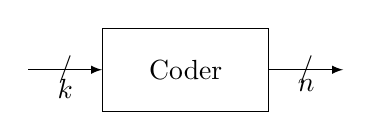
\begin{tikzpicture}[
                    node distance=2cm,
                    >=latex
                    ]

                    \node [coordinate] (input) {};
                    \node [draw, rectangle,right of = input, minimum height=3em, minimum width=6em] (block) {Coder};
                    \node [coordinate, right of = block] (output) {};
                    
                    \draw[draw,->] (input) -- node[midway]{$/$} node[below]{$k$} (block);
                    \draw[->] (block) -- node[midway]{$/$} node[below]{$n$} (output);
                \end{tikzpicture}    
            \label{Def codice forma sistematica}
            \end{figure}
            \begin{figure}[H]
                \centering 
                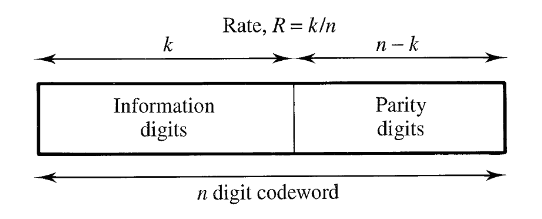
\includegraphics[width = 8cm]{media/forma sistematica.png}
            \label{matrice forma sistematica}
            \end{figure}
            \paragraph{Esempio Codice a ripetizione:}
            $R = \frac{1}{3},\ k=1,\ n=3$
            \begin{table}[H]
                \centering
                \begin{tabular}{|c|c|}
                \hline
                Bit i  ingresso & Parola codificata \\ \hline
                0               & {[}000{]}         \\ \hline
                1               & {[}111{]}         \\ \hline
                \end{tabular}
            \end{table}
            La matrice generatrice del codice è $G = [111]$, e la distanza minima $d_{min} = 3$\\

            \paragraph{Esempio Codice a controllo di parità:}
            $R = \frac{7}{8},\ k=7,\ n=8$, ogni 7 bit ne aggiunge uno di controllo di parità, 1 se il numero di "1" è dispari,
            0 se il numero di "1" è pari.


            \noindent La matrice generatrice del codice:
            \[
                G = [I_7,1_7]
            \]
            \noindent La distanza minima è $d_{min} = 2$, se cambio uno dei 7 bit della parola
            cambio automaticamente il bit di parità, quindi cambiare 1 bit in realtà ne cambia 2.\\

            \noindent Il prodotto $u\dotproduct 1_7 = \sum_{i=1}^{7}u_i$, può essere scritto come una soma modulo 2, vale 0 se il numero di 
            occorrenze di "1" è pari e 1 altrimenti. Non facciamo altro che calcolare il bit di parità della parola $u$.
            
            \paragraph{Definizione:} Due codici lineari $\mathcal{C}_1(k,n)$ e $\mathcal{C}_2(k,n)$ in $GF(2)$ sono equivalenti se uno è ottenuto dall'altro
            attraverso una permutazione delle posizioni del codice.

            \paragraph{Teorema:} Due matrici generatrici $G_1$ e $G_1$ in $GF(2)$ generano due codici equivalenti se una può essere ottenuta dall'altra
            da una sequenza di operazioni come:
            \begin{itemize}
                \item Permutazione delle righe.
                \item Combinazione lineare delle righe.
                \item Permutazione delle colonne.
            \end{itemize}
            
            \paragraph{Teorema:} Qualsiasi codice lineare a blocchi è equivalente ad un codice in forma sistematica.

            \paragraph{Proprietà degli spazi:}
            \begin{itemize}
                \item {
                    Dato il sottospazio $\mathcal{C} \subset \mathcal{V}_n$ di dimensione $k$, esiste un sottospazio ortogonale (null space)
                    $\mathcal{C}^\perp \subset \mathcal{V}_n$ di dimensione $n-k$ definito da una matrice $H\in (n-k) \times n$:
                    \[
                        GH^T = 0_{n-k}  
                    \]
                }
                \item {
                    La base di $\mathcal{C}^\perp$ è costituita dalle $n-k$ righe della matrice $H$, per cui ogni elemento $t\in \mathcal{C}^\perp$ può 
                    essere rappresentato:
                    \[
                        t = vH = \sum_{i=1}^{n-k}v_ih_i  
                    \]
                }
                \item {
                    Per ogni $x\in \mathcal{C}$ e per ogni $t\in \mathcal{C}^\perp$ si ha:
                    \[
                        xt^T = uGH^Tv^T = 0
                    \]  
                }
            \end{itemize}
        \subsubsection{Matrice di controllo di parità}\label{Matrice di controllo di parita}\index{Matrice di controllo di parità}
            La matrice $H$ è la matrice di controllo di parità del codice. Per costruzione $\forall x \in \mathcal{C}$ vale:
            \begin{gather}
                    xH^T = uGH^T = 0 \nonumber \\
                    H\in (n-k) \times n\nonumber 
            \end{gather}
            La matrice $H$ non è unica, ma se il codice è sistematico posso ricavarla in un'altra forma:
            \begin{gather}
                H = [P^T,I_{n-k}] = 0 \nonumber \\
                H\in (n-k) \times n,\ I\in (n-k)\times (n-k),\ P^T\in (n-k) \times k \nonumber
            \end{gather}
            Se fosse $\neq 0$ ciò che è stato ricevuto non è una parola di codice.
            
            \paragraph{Esempio codice a ripetizione e controllo di parità:}
                $R = \frac{1}{3},\ k=1,\ n=3,\ n-k=2$ ho la matrice a controllo di parità:
                \[
                    H= [P^T,I_2] =
                        \begin{bmatrix}
                        1 & 1 & 0\\
                        1 & 0 & 1
                        \end{bmatrix}  
                \]  
                Per un codice con $R = \frac{7}{8},\ k=7,\ n=8,\ n-k=1$ la matrice a controllo di parità:
                \[
                    H= [P^T,I_1] = 1_8^T
                \]
        \subsubsection{Proprietà dei codici a blocco}
            \paragraph{Teorema:} La distanza minima del codice a blocco $\mathcal{C}(k,n)$ si può calcolare come il 
            peso di Hamming minimo tra tutte le parole di codice:
            \begin{align}
                d_{min}(\mathcal{C}) &= \underset{x_i,x_j\in\mathcal{C}}{\min} d_H(x_i,x_j) = \underset{x_i,x_j\in\mathcal{C}}{\min} d_H(x_i+x_j,x_j+x_j)\nonumber \\
                                     &= \underset{x_i,x_j\in\mathcal{C}}{\min} d_H(x_i+x_j,0_{1,n}) \overset{[x_i+x_j\in\mathcal{C}]}{\Rightarrow} \underset{x_i\in\mathcal{C}}{\min}\ w(x_i)\nonumber
            \end{align}
            \paragraph{Capacità di rivelare errori (Error Detection):}
                Su un canale $BSC$ senza memoria (\ref{BSC system moretti}), la $n-upla\ y$ a valle del decisore può essere rappresentata:
                \[
                    y=x+e  
                \] 
                Dove $e$ è il vettore di errori introdotto dal canale, se il canale non introduce errori: $e = 0_{1,n}$
                Sia $x$ la parola di codice trasmessa e $y=x+e$ la corrispondente sequenza di $n$ bit ricevuta. supponiamo che il canale 
                introduca un numero di errori:$w(e) > 0$, si dice:
                \begin{itemize}
                    \item {
                        Errore Rivelabile\index{Errore Rivelabile}: se $y$ non è una parola di codice, $y\notin\mathcal{C}(k,n) $
                    }
                    \item {
                        Errore Non Rivelabile\index{Errore Non Rivelabile}: se $y$ è una parola di codice ma non quella trasmessa, $w(e) \geq d_{min}$ 
                    }
                \end{itemize} 
                \subparagraph{Teorema:} Il codice $\mathcal{C}(k,n)$ è in grado di rivelare con certezza fino a $d_{min}-1$ errori.
                \begin{itemize}
                    \item {
                        Se $d(x,y)<d_{min}$: $y$ non può essere una parola di codice, altrimenti vorrebbe dire che esistono due parole di codice la cui distanza 
                        è minore di $d_{min}$.
                    }
                    \item {
                        Se $d(x,y)=d_{min}$: esiste almeno una parola di codice $c\in\mathcal{C}(k,n),\ c \neq x$ tale che $d(x,c)=d_{min}$, se $y=c$ l'errore non 
                        può essere rivelato. 
                    }
                \end{itemize}
            \paragraph{Strategia di decodifica a massima verosimiglianza:}
                Sia $y$ il vettore ricevuto a seguito della trasmissione su $BSC$ , la strategia di decodifica a massima verosimiglianza (ML, maximum likelihood) 
                consiste nel trovare il vettore $\hat{x}$ che, tra tutte le $2^k$ possibili parole di codice $x$, massimizza la probabilità condizionata 
                $P(y|x)$:
                \[
                    \hat{x} = \arg \underset{x\in\mathcal{C}}{\max}\ P(y|x)
                \]
                Poiché gli eventi di errore sono indipendenti da bit a bit, posso riscrivere la probabilità condizionata come il prodotto delle probabilità condizionate
                ottenute per ciascun bit trasmesso:
                \[
                    P(y|x) = \prod_{\ell=1}^{n} P(y_\ell|x_\ell)
                \]
                Lavorando in $GF(2)$ la probabilità $P(y_\ell|x_\ell)$ può assumere solo 2 valori:
                \[
                    P(y_\ell|x_\ell) = 
                    \begin{cases}
                        1-p &se\ P(y_\ell =x_\ell|x_\ell)\nonumber \\    
                        p   &se\ P(y_\ell \neq x_\ell|x_\ell)\nonumber     
                    \end{cases}
                \] 
                Osservazione: La distanza di Hamming $d_H(x,y)$ misura il numero di posizione diverse tra $x$ e $y$, quindi $n-d_H(x,y)$ misura il numero di posizioni
                uguali tra $x$ e $y$.

                La probabilità $P(y|x)$ si calcola:
                \[
                    P(y|x) = p^{d_H(x,y)}(1-p)^{n-d_H(x,y)} =(1-p)^{n}\left(\frac{p}{1-p}\right)^{d_H(x,y)} 
                \]
                Mi interessa scegliere un $x$ che massimizza $\left(\frac{p}{1-p}\right)^{d_H(x,y)}$, è un valore $<1$:
                \begin{itemize}
                    \item {
                        Se ho la $d_H(x,y)$ piccola ho la probabilità minore di errore.
                    }
                    \item {
                        Se ho la $d_H(x,y)$ alta ho la probabilità di errore alta.
                    }
                \end{itemize}
                
            \paragraph{Decisione a massima verosimiglianza:}\label{Decisione a massima verosomiglianza}\index{Decisione a massima verosomiglianza}
                La parola di codice decisa $\hat{x}$ è quella che minimizza la distanza dalla parola $y$ ricevuta:
                \[
                    \hat{x} = \arg \underset{x\in\mathcal{C}}{\max}\ P(y|x) = \arg \underset{x\in\mathcal{C}}{\min}\ d_H(y,x)
                \]
                Scelgo $x$ tale che mi dia la minima distanza
                \subparagraph{Ricevitore ML ottimo:}\index{Ricevitore ML ottimo} Il ricevitore ML ottimo è il ricevitore a distanza minima, il ricevitore
                che associa alla sequenza di $n$ bit ricevuta $y$, la parola di codice $x$ che minimizza la $d_H(y,x)$.
                \subparagraph{Ricevitore ML error correction:}\index{Ricevitore ML error correction} Il ricevitore ML è in grado di correggere con successo tutti quegli errori
                $e$ per cui la parola ricevuta $y = x+e$ è comunque più vicina alla parola trasmessa $x$ che a qualsiasi altra parola del codice.
                
                Per ogni vettore $v\in\mathcal{V}_n$ e un raggio $r$ esiste una "sfera" di raggio $r$ i cui elementi sono tutti quei vettori in $\mathcal{V}_n$ che hanno
                distanza di Hamming da $v$ minore o uguale a $r$

                \begin{figure}[H]
                    \centering 
                    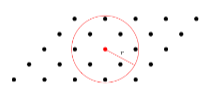
\includegraphics[width = 4cm]{media/sfera di amming.png}
                \label{sfera di Hamming}
                \end{figure}
                Se adottiamo un ricevitore ML, il numero massimo di errori che il codice $\mathcal{C}(k,n)$ è in grado di correggere è il massimo raggio $t$ per cui le sfere centrate nelle 
                parole di codice di $\mathcal{C}(k,n)$ sono tutte tra loro disgiunte.
            \paragraph{Capacità di correggere errori (Error Correction):}
                \subparagraph{Teorema:}\begin{sloppypar}
                   Un codice lineare a blocco può correggere fino a ${t_{max} = \left\lfloor \frac{d_{min}-1}{2} \right\rfloor}$ errori: $2t_{max}+1 \leq d_{min} \leq 2t_{max}+2$.
                \end{sloppypar}
                    
                \begin{sloppypar}
                    La condizione per cui le sfere di raggio $t$ che circondano le parole di codice siano disgiunte è che ${2t_{max} < d_{min}\Rightarrow t_{max} < \frac{d_min}{2}}$.
                    Altrimenti se fosse  ${2t_{max} \geq d_{min}}$ ci sarebbero almeno due parole $x_1$ e $x_2$ la cui distanza ${d_H(x_1,x_2) = d_{min} < 2t_{max} }$ e le due sfere di raggio
                    $t$ avrebbero almeno un punto in comune.
                \end{sloppypar}
                
                \begin{sloppypar}
                    Consideriamo il codice $\mathcal{C}(k,n)$ che ha una certa $d_{min}$ e $t_{max}$ tale che ${2t_{max}+1 \leq d_{min}}$. Sia $x\in\mathcal{C}(k,n)$ la parola trasmessa,
                    ${y = x+e}$ la corrispondente sequenza di $n$ bit ricevuta e $c\in\mathcal{C}(k,n)$ un'altra generica parola di codice. Grazie alla disuguaglianza triangolare ho:
                    \[
                        d_H(x,y) + d_H(c,y) \geq d_H(x,c) \Rightarrow d_H(c,y) \leq d_H(x,c) - d_H(x,y)  
                    \]
                    per ipotesi ho anche:
                    \[
                        d_H(x,c) \geq d_{min} \geq 2t_{max}+1 
                    \]
                    Supponiamo che il canale introduca un certo numero di errori ${t\leq} t_{max}$, così da avere $d_H(x,y) = t$:
                    \[
                        d_H(c,y) \geq 2t_{max}+1 -t > t_{max} \geq t = d_H(x,y)   
                    \]   
                \end{sloppypar}
                
    \subsection{Codici di Hamming}
        I codici di Hamming $\mathcal{C}_H(m)$ sono definiti a partire da un parametro: $m \geq 2$
        \[
            n = 2^m-1,\ k = 2^m-m-1 = n-m
        \]
        \subparagraph{Matrice di controllo di parità:} per definizione la matrice $H \in (n-k)\times n$, ma per i codici di Hamming la matrice $H$ ha dimensione:
        $H \in m\times (2^m-1)$.

        \subparagraph{Matrice di parità:} Per un codice di Hamming sistematico la matrice di parità $P\in k \times m$ viene costruita così che le colonne di $H = [P^T,I_{n-k}]$
        siano tutte le possibili $2^m-1$ combinazioni di $m$ bit (esclusa la $n-upla$ di tutti 0)

        \subsubsection{Il codice $\mathcal{C}_H(2)$}
            \begin{sloppypar}
                Il codice a ripetizione ${R=\frac{1}{3}}$ con ${m=2\Rightarrow n=3,\ k=1}$ ha come matrice di controllo di parità $H$:
                \[
                    H = \begin{bmatrix}
                            1  & 1 & 0 \\
                            1  & 0 & 1 \\
                        \end{bmatrix} 
                \]
                Che è la matrice corrispondente a un codice di Hamming $\mathcal{C}_H(2)$, poiché rappresenta tutte le possibili combinazioni di 2 bit
            \end{sloppypar}

        \subsubsection{Il codice $\mathcal{C}_H(3)$}
        \begin{gather}
            m=3,\ n=7,\ k=4,\ R=\frac{4}{7} \nonumber \\
            H = \begin{bmatrix}
                1 & 0 & 1 & 0 & 1 & 0 & 1\\
                0 & 1 & 1 & 0 & 0 & 1 & 1\\
                0 & 0 & 0 & 1 & 1 & 1 & 1
            \end{bmatrix}  \nonumber
        \end{gather}
        Posso ricavare la matrice generatrice $G$ scrivendo la matrice $H$ come se l'avessi ottenuta da una matrice $G\in k \times n$ di un codice sistematico (\ref{Matrice di controllo di parita}):
        \[
            H = [P^T,I_{n-k}] =\begin{bmatrix}
                                 1  & 1 & 0 & 1 & | & 1  & 0 & 0\\
                                 1  & 0 & 1 & 1 & | & 0  & 1 & 0\\
                                 0  & 1 & 1 & 1 & | & 0  & 0 & 1
                            \end{bmatrix} 
        \]
        La cui matrice generatrice con $I \in k \times k$ é:
        \[
            G = [I_{k},P] =\begin{bmatrix}
                                 1  & 0 & 0 & 0 & | & 1  & 1 & 0\\
                                 0  & 1 & 0 & 0 & | & 1  & 0 & 1\\
                                 0  & 0 & 1 & 0 & | & 0  & 1 & 1\\
                                 0  & 0 & 0 & 1 & | & 1  & 1 & 1
                            \end{bmatrix} 
        \]
        Possiamo vedere come la matrice di parità faccia controlli su combinazioni diverse di bit in ingresso $p = uP$:
        \begin{gather}
            p_1 = u_1+u_2+u_4 \nonumber\\
            p_2 = u_1+u_3+u_4 \nonumber\\
            p_3 = u_2+u_3+u_4 \nonumber
        \end{gather}
        Il vettore di uscita dal codificatore sarà quindi $x = uG = [u,p_1,p_2,p_3]$, tale matrice di parità ci permette di aumentare la distanza di Hamming
        tra le parole
        \subparagraph{Distanza minima:} La distanza minima di un qualsiasi codice di Hamming $\mathcal{C}_H(m)$ è $d_{min}(\mathcal{C}_H(m)) = 3$.

        \noindent Dimostrazione: 
        \begin{enumerate}
            \item {
                $d_{min} = \underset{x\in\mathcal{C}}{\min}\ w(x)$  
            }
            \item {
                $x\in\mathcal{C}\ se\ xH^T= 0$ e le colonne di $H$ sono tutte le possibili combinazioni dei bit $m$ bit
            }
        \end{enumerate}
        Perché $3$ è il numero minimo di colonne che mi permette di ottenere $0$ ($2$), quindi $d_{min}(\mathcal{C}_H(m)) = 3$.
        
        %Ne consegue che aumentando il numero di bit trasmessi diminuisco la ridondanza, ma la mia distanza di Hamming rimane sempre la stessa.
    \subsection{Decodifica per codici a blocco}
        Dato il vettore ricevuto:
        \[
            y = x+e
        \]
        Il decisore ottimo selezione la parola di codice $\hat{x}$:
        \[
            \hat{x} = \arg \underset{x\in\mathcal{C}}{\max}\ P(y|x) = \arg \underset{x\in\mathcal{C}}{\min}\ d_H(y,x)   
        \]
        Per ottenere $\hat{x}$ è necessario fare $2^k$ confronti tra il vettore ricevuto $y$ e tutte le parole di codice $\mathcal{C}(k,n)$, 
        la complessità cresce esponenzialmente con $k$.

        Un approccio alternativo è quello di osservare il vettore errore e la probabilità condizionata:
        \begin{gather}
            y= x+e \Rightarrow x = y+e,\ e = y-x\nonumber\\
            P(x|y) = P(x+e|x) = P(e|y+e\in\mathcal{C})\nonumber
        \end{gather}
        Posso ottenere la stima di $x$ come:
        \[
            \hat{x} = \arg \underset{x\in\mathcal{C}}{\max}\ P(y|x) =y+ \arg \underset{e}{\max}\ P(e|y+e\in\mathcal{C})   
        \]
        Invece di stimare $\hat{x}$ si stima il vettore $\hat{e}$ più probabile
        \begin{align}
            \hat{e} &= \arg \underset{e}{\max}\ P(e|y+e\in\mathcal{C}) = \arg \underset{e|y+e\in\mathcal{C}}{\max}\ p^{w(e)}(1-p)^{n-w(e)} \nonumber \\
                    &= \arg \underset{e|y+e\in\mathcal{C}}{\max}\ \left(\frac{1-p}{p}\right)^{-w(e)} = \arg \underset{e|y+e\in\mathcal{C}}{\min}\ w(e)  \nonumber 
        \end{align}
        La decodifica sceglie tra tutti i possibili vettori errore $e$ tali che $y+e\in\mathcal{C}$ quello che ha il peso di Hamming minimo, cioè il minimo numero di 
        errori (Massima Verosimiglianza). Una volta stimato $\hat{e}$:
        \[
            \hat{x} = y-\hat{e} = y+\hat{e} = x+(\hat{e}+e)=
            \begin{cases}
                x &se\ \hat{e} = e\nonumber\\    
                x_1\neq x &se\ \hat{e} \neq e\nonumber    
            \end{cases}     
        \]
        \subsubsection{Coset}
            Sia $\mathcal{C}(k,n)$ un codice a blocco e sia $v\in \mathcal{V}_n$ un vettore di $n$ cifre binarie, si definisce $coset$ di
            $\mathcal{C}(k,n)$ individuato da $v$ l'insieme:
            \[
                C_v = C+v=\{ x+v: x\in\mathcal{C} \}
            \]
        \subsubsection{Proprietà dei coset}
            \begin{enumerate}
                \item {Qualsiasi vettore in $\mathcal{V}_n$ appartiene a un coset di $\mathcal{C}(k,n)$}
                \item {Ciascun coset contiene $2^k$ elementi}
                \item {Due coset o sono coincidenti o hanno intersezione nulla}
                \item {Ci sono $2^{n-k}$ coset distinti}
                \item {Se $v_1$ e $v_2$ appartengono allo stesso coset, $v_1 + v_2 \in \mathcal{C}(k,n)$ è una parola di codice}
            \end{enumerate}
            \paragraph{Esempio di coset:}
                \begin{sloppypar}
                    Sia ${\mathcal{C}(2,3) = \{000,101,010,111\}}$. I coset di ${\mathcal{C}(2,3)}$: 
                \end{sloppypar}
                \begin{align}
                    \mathcal{C} + 000 = \{000,101,010,111\} = \mathcal{C}_0 \\
                    \mathcal{C} + 001 = \{001,100,011,110\} = \mathcal{C}_1 \\
                    \mathcal{C} + 010 = \{010,111,000,101\} = \mathcal{C}_0 \\
                    \mathcal{C} + 011 = \{011,110,001,100\} = \mathcal{C}_1 \\
                    \mathcal{C} + 100 = \{100,001,110,011\} = \mathcal{C}_1 \\
                    \mathcal{C} + 101 = \{101,000,111,010\} = \mathcal{C}_0 \\
                    \mathcal{C} + 110 = \{110,011,100,001\} = \mathcal{C}_1 \\
                    \mathcal{C} + 111 = \{111,010,101,000\} = \mathcal{C}_0 
                \end{align}
                Il numero di coset è $2^{n-k} = 2^{3-2} =2$.

            Si possono applicare i coset per la decodifica: $y=x+e$ dalla definizione di coset discende che i vettori $e$ e $y$
            appartengono allo stesso coset $\mathcal{C}_y$ e che i coset $\mathcal{C}_e$ e $\mathcal{C}_x$ sono coincidenti. Grazie alla proprietà
            dei coset la somma di qualsiasi elemento di $\mathcal{C}_y$ con $y$ individua una parola di codice. Il vettore $e$ va scelto fra gli elementi
            di $\mathcal{C}_y$, la regola di decisione diventa:
            \[
                \hat{e} = \arg \underset{e}{\max}\ P(e|y+e\in\mathcal{C}) = \arg \underset{e\in\mathcal{C}_y }{\max}\ P(e) =\arg \underset{v\in\mathcal{C}_y }{\max}\ w(v)
            \] 
            Tra tutti i $2^k$ possibili vettori di $\mathcal{C}_y$, il principio di massima verosimiglianza dice che devo scegliere quello di peso minimo.
        \subsubsection{Algoritmo di decodifica}
            \begin{enumerate}
                \item Avendo ricevuto il vettore $y$ si trova un coset di appartenenza $\mathcal{C}_y$.
                \item {Si identifica il coset leader, la parola di peso minimo del coset $\mathcal{C}_y$, che è anche la parola di peso minimo del 
                coset di $\mathcal{C}_e$.}
                \item Il coset leader è la stima del vettore di errore $\hat{e}$
            \end{enumerate}
            \paragraph{Esempio di decodifica utilizzando i coset:}
                    Sia ${\mathcal{C}(2,4) = \{0000,1011,0101,1110\}}$ con $d_{min} = 2$, ho i coset: 
                \begin{align}
                    \mathcal{C} + 0000 = \{0000,1011,0101,1110\} \\
                    \mathcal{C} + 0001 = \{0001,1010,0100,1111\} \\
                    \mathcal{C} + 0010 = \{0010,1001,0111,1100\} \\
                    \mathcal{C} + 1000 = \{1000,0011,1101,0110\} 
                \end{align}
                Il numero di coset è $2^{n-k} = 2^{4-2} =4$. Il coset (2) non so quale coset leader scegliere hanno lo stesso peso di Hamming, ci
                troviamo in questo poiché la $d_{min}$ è molto bassa e ho il $50\%$ di possibilità di sbagliare se il codice ricevuto capita in questo coset.
                Decodifichiamo:
                \begin{itemize}
                    \item {$y=[1101]\Rightarrow y\in (4),\text{coset leader:} [1000]\ \hat{x}=y+1000=0101$}
                    \item {$y=[1111]\Rightarrow y\in (2),\text{coset leader:} [0001] \vee [0100] \ \hat{x}=y+0001=1110$}
                \end{itemize}
        \subsubsection{Decodifica mediante sindrome}
            Si definisce sindrome di $y$ il vettore $s$ ottenuto dal prodotto di $y$ con la matrice di controllo di parità:
            \[
                s = yH^T = (x+e)H^T = xH^T+eH^T = eH^T    
            \]
            \paragraph{Proprietà:}
                \begin{itemize}
                    \item {
                        Tutti i membri di uno stesso coset hanno la stessa sindrome
                    }
                    \item {
                        $s \in 1 \times (n-k)$
                    }
                    \item {
                        Le $2^{n-k}$ sindromi sono associate ai $2^n-k$ diversi coset del codice $\mathcal{C}(k,n)$
                    }
                    \item {
                        Ciascuna sindrome è associata ai $2^k$ pattern di errore appartenenti allo stesso coset.
                    }
                \end{itemize}
            \paragraph{Procedura di decodifica:}
                \begin{enumerate}
                    \item {Calcola la sindrome $s = yH^T$}
                    \item {Associa la sindrome al coset leader corrispondente $s\rightarrow e_{CL}(s)$}
                    \item {Corregge l'errore sommando il coset leader alla $n-upla\ y$}
                \end{enumerate}
                La parola $\hat{x}$ è una parola di codice:
                \[
                    \hat{x}H^T= (y+e_{CL}(s))H^T = s+s =0   
                \]
                e per costruzione la parola di codice $\hat{x}$ minimizza la distanza di Hamming da $y$
        \subsubsection{Decodifica a sindrome: Codici di Hamming $m=3$}
            \begin{sloppypar}
                Il codice ha $d_{min} = 3$ ed è in grado di correggere esattamente un errore: ${t_{max} = \left\lfloor \frac{d_{min}-1}{2}\right\rfloor = 1}$. Si sceglie la matrice $H$
                in maniera che la tabella di decodifica associ alla sindrome il pattern di errore a peso 1 in cui il bit
                messo a 1 sia nella posizione corrispondente alla conversione della sindrome in decimale.
            \end{sloppypar}
            \begin{table}[H]
                \subfloat[Codice non sistematico]{
                    \begin{tabular}{cc}
                        \hline
                        Sindrome  & Coset Leader  \\ \hline
                        {[}000{]} & {[}0000000{]} \\
                        {[}100{]} & {[}1000000{]} \\
                        {[}010{]} & {[}0100000{]} \\
                        {[}110{]} & {[}0010000{]} \\
                        {[}001{]} & {[}0001000{]} \\
                        {[}101{]} & {[}0000100{]} \\
                        {[}011{]} & {[}0000010{]} \\
                        {[}111{]} & {[}0000001{]} \\ \hline
                        \end{tabular}
                }
                \hfill
                \subfloat[Codice sistematico]{
                    \begin{tabular}{cc}
                        \hline
                        Sindrome  & Coset Leader  \\ \hline
                        {[}000{]} & {[}0000000{]} \\
                        {[}100{]} & {[}0000100{]} \\
                        {[}010{]} & {[}0000010{]} \\
                        {[}110{]} & {[}1000000{]} \\
                        {[}001{]} & {[}0000001{]} \\
                        {[}101{]} & {[}0100000{]} \\
                        {[}011{]} & {[}0010000{]} \\
                        {[}111{]} & {[}0001000{]} \\ \hline
                    \end{tabular}
                }
            \end{table}
        \subsubsection{Esempio di decodifica}
            Un codice lineare a blocchi ha la seguente matrice di controllo di parità:
            \[
                H=
                    \begin{bmatrix}
                    1 & 0 & 1 & 1 & 0 & 0\\
                    1 & 1 & 0 & 0 & 1 & 0\\
                    0 & 1 & 1 & 0 & 0 & 1
                    \end{bmatrix}  
            \]  
            \begin{enumerate}
                \item {Determinare la matrice generatrice:
                    \begin{itemize}
                        \item{ 
                            Ci accorgiamo che il codice è in forma sistematica: abbiamo la matrice identica 
                            \[
                                H=
                                    \begin{bmatrix}
                                    1 & 0 & 1 & | & 1 & 0 & 0\\
                                    1 & 1 & 0 & | & 0 & 1 & 0\\
                                    0 & 1 & 1 & | & 0 & 0 & 1
                                    \end{bmatrix}  
                            \]  
                            Allora la forma $H = [P^T,I_{n-k}]$, e la matrice parità ha forma $G = [I_k,P]$:
                            \[
                                G=
                                    \begin{bmatrix}
                                    1 & 0 & 0 & | & 1 & 1 & 0 \\
                                    0 & 1 & 0 & | & 0 & 1 & 1 \\
                                    0 & 0 & 1 & | & 1 & 0 & 1 
                                    \end{bmatrix}  
                            \]
                        }
                    \end{itemize}
                }
                \item {Decodificare la parola $y = [110110]$ ed identificare la parola di codice trasmessa:
                    \begin{itemize}
                        \item {Verifichiamo se è stato introdotto errore, calcoliamo la sindrome $s = yH^T$ e calcoliamone il prodotto in $G(2)$:
                        \[
                            yH^T=
                                \begin{bmatrix}
                                1 & 1 & 0 & 1 & 1 & 0
                                \end{bmatrix}
                                \begin{bmatrix}
                                1 & 1 & 0 \\ 
                                0 & 1 & 1 \\ 
                                1 & 0 & 1 \\ 
                                1 & 0 & 0 \\
                                0 & 1 & 0 \\
                                0 & 0 & 1 
                                \end{bmatrix} =
                                    \begin{bmatrix}
                                    0 & 1 & 1 
                                    \end{bmatrix}   
                        \]
                        }
                        \item {Essendo il codice diverso da $0$ è stato introdotto un errore, devo trovare la stima dell'errore: $y=x+e$ sia una parola di codice. 
                            La sindrome identifica un coset e di conseguenza l'errore a esso associato. Ma mi accorgo che $[011]$ (sindrome) corrisponde a una riga della matrice di controllo di parità $H$, quindi posso selezionare la riga moltiplicandola per un vettore 
                            riga composto da zeri tranne un uno per la riga che voglio selezionare (questo avrà peso 1):
                            
                            \begin{align}
                                    \hat{x} &= y + \hat{e} =  (y + \hat{e})H^T=y H^T+ \hat{e}H^T= s+s =0 \nonumber \\
                                    &\begin{bmatrix}
                                        0 & 1 & 0 & 0 & 0 & 0
                                        \end{bmatrix}
                                        \begin{bmatrix}
                                        1 & 1 & 0 \\ 
                                        0 & 1 & 1 \\ 
                                        1 & 0 & 1 \\ 
                                        1 & 0 & 0 \\
                                        0 & 1 & 0 \\
                                        0 & 0 & 1 
                                        \end{bmatrix} = 0  \nonumber
                            \end{align}  
                        }
                        \item {Abbiamo quindi 
                        \begin{gather}
                            \hat{y} =\begin{bmatrix}
                                1 & 1 & 0 & 1 & 1 & 0
                                \end{bmatrix} \nonumber \\
                            \hat{e} = \begin{bmatrix}
                                0 & 1 & 0 & 0 & 0 & 0
                                \end{bmatrix}\nonumber \\
                            \hat{x} = \begin{bmatrix}
                                1 & 0 & 0 & 1 & 1 & 0
                                \end{bmatrix}\nonumber \\
                            xH^T=
                                \begin{bmatrix}
                                1 & 0 & 0 & 1 & 1 & 0
                                \end{bmatrix}
                                \begin{bmatrix}
                                1 & 1 & 0 \\ 
                                0 & 1 & 1 \\ 
                                1 & 0 & 1 \\ 
                                1 & 0 & 0 \\
                                0 & 1 & 0 \\
                                0 & 0 & 1 
                                \end{bmatrix} =
                                    \begin{bmatrix}
                                    0 & 0 & 0 
                                    \end{bmatrix}\nonumber   
                    \end{gather}
                        }
                        \item {Abbiamo decodificato e siamo arrivati a una parola di codice. Evviva! UwU ti meriti un bacino.}
                    \end{itemize}
                }
            \end{enumerate}
            \paragraph{Esempio con codici di Hamming:} 

    \subsection{Codici Ciclici}
        \paragraph{Shift Ciclico:}\label{shift ciclico}
            \begin{sloppypar}
                Dato il vettore ${v = [v_0,\dots,v_{n-1}]\in \mathcal{V} = G(2)^n}$ indichiamo con $v^{(i)}$ il vettore ottenuto da $v$ applicando uno 
                \emph{shift ciclico} di $i$ posizioni a destra:
                \[
                    v^{(i)} = [v_{n-i},v_{n-i+1}, \dots, v_{n-1},v_0,v_1,\dots, v_{n-i-1}]    
                \]     
            \end{sloppypar}
        \subsubsection{Definizione di Codice Ciclico}
            Un codice lineare $\mathcal{C}(k,n)$ si definisce \emph{ciclico} se data una generica parola di codice $x\in \mathcal{C}(k,n)$ ogni suo
            shift ciclico $x^{(i)}\in \mathcal{C}(k,n)$. Sono codici a correzione d'errore che hanno proprietà algebriche che rendono sia la rivelazione che la correzione
            di errore efficienti.
            \paragraph{Esempi - Codici Ciclici:}
                \begin{itemize}
                    \item {
                        $\mathcal{C}(2,3) = \{000,110,101,011\}$
                    }
                    \item {
                        $\mathcal{C}(2,4) = \{0000,1010,0101,1111\}$ 
                    }
                    \item {
                        $\mathcal{C}(4,7)$:\label{codice 47}
                        \begin{table}[H]
                            \centering
                            \begin{tabular}{ccl}
                            \cline{1-3}
                            Messaggio  & Vettori di Codice & Polinomi di codice \\ \cline{1-3}
                            {[}0000{]} & {[}0000000{]}     &$0=                                    0\dotproduct g_{(D)}$\\
                            {[}1000{]} & {[}1101000{]}     &$1+D+D^3 =1                             \dotproduct g_{(D)}$\\
                            {[}0100{]} & {[}0110100{]}     &$D+D^2+D^4 =                           D\dotproduct g_{(D)}$\\
                            {[}1100{]} & {[}1011100{]}     &$1+D^2+D^3+D^4 =                   (1+D)\dotproduct g_{(D)}$\\
                            {[}0010{]} & {[}0011010{]}     &$D^2+D^3+D^5 =                       D^2\dotproduct g_{(D)}$\\
                            {[}1010{]} & {[}1110010{]}     &$1+D+D^2+D^5 =                   (1+D^2)\dotproduct g_{(D)}$\\
                            {[}0110{]} & {[}0101110{]}     &$D+D^3+D^4+D^5 =                 (D+D^2)\dotproduct g_{(D)}$\\
                            {[}1110{]} & {[}1000110{]}     &$1+D^4+D^5 =                   (1+D+D^2)\dotproduct g_{(D)}$\\ 
                            {[}0001{]} & {[}0001101{]}     &$D^3+D^4+D^6 =                       D^3\dotproduct g_{(D)}$\\
                            {[}1001{]} & {[}1100101{]}     &$1+D+D^4+D^6 =                   (1+D^3)\dotproduct g_{(D)}$\\
                            {[}0101{]} & {[}0111001{]}     &$D+D^2+D^3+D^6 =                 (D+D^3)\dotproduct g_{(D)}$\\
                            {[}1101{]} & {[}1010001{]}     &$1+D^2+D^6 =                   (1+D+D^3)\dotproduct g_{(D)}$\\
                            {[}0011{]} & {[}0010111{]}     &$D^2+D^4+D^5+D^6 =             (D^2+D^3)\dotproduct g_{(D)}$\\
                            {[}1011{]} & {[}1111111{]}     &$1+D+D^2+D^3+D^4+D^5+D^6 =   (1+D^2+D^3)\dotproduct g_{(D)}$\\
                            {[}1111{]} & {[}1001011{]}     &$1+D^3+D^5+D^6 =           (1+D+D^2+D^3)\dotproduct g_{(D)}$
                            \end{tabular}
                        \end{table}
                    }
                \end{itemize}
        \subsubsection{Rappresentazione algebrica di un codice ciclico}
            A ciascun vettore $v = [v_0,\dots,v_{n-1}]\in \mathcal{V}$ è possibile associare un polinomio definito in $GF(2)$:
            \[
                v_{(D)} = v_0 + v_1 D+\dots+ v_{n-1}D^{n-1}    
            \]
            \paragraph{Definizione:} se $x_{(D)} \leftrightharpoons x\in \mathcal{C}(k,n) \Rightarrow$ si dice
            che $x_{(D)}$ è in $\mathcal{C}(k,n)$
            \paragraph{Proprietà:} Uno \emph{shift ciclico} \ref{shift ciclico} di $i$ posizioni del vettore $v$ è equivalente a moltiplicare
            il polinomio $v_{(D)}$ per $D^i$ modulo $(D^n-1)$:
            \[
                v^{(i)} \rightleftharpoons \mod\{D^iv_{(D)},(D^n-1)\}    
            \]
            il modulo tra polinomi è il resto della divisione tra polinomi, il grado quindi sarà sempre minore o uguale a $n$. Fissando 
            $i=1$ il polinomio diventa:
            \begin{align}
                Dv_{(D)} &= v_0D+v_1D^2+ \dots +v_{n-1}D^n \nonumber \\
                         &\overset{\pm v_{n-1}}{=} v_{n-1}+v_0D+v_1D^2+ \dots +\underset{v_{n-1}(D^n-1)}{\underbrace{v_{n-1}D^n - v_{n-1}}}\nonumber \\
                         &= v_{n-1}+v_0D+v_1D^2+ \dots + v_{n-2}D^{n-1}+v_{n-1}(D^n-1)\nonumber 
            \end{align}        
            facendone il modulo:
            \[
                \mod\{D^iv_{(D)},(D^n-1)\}=v_{n-1}+v_0D+v_1D^2+ \dots + v_{n-2}D^{n-1} \rightleftarrows v^{(1)}
            \]
            ho ottenuto il codice shiftato di una posizione, analogamente si può dimostrare che:
            \[
                D^iv_{(D)} = q_{(D)}(D^n-1) +v_{n-i}+v_0D+v_1D^2+ \dots +v_{n-i-1}D^{n-1}\nonumber \\
            \]
            quindi il modulo ci fornisce lo shift:
            \[
                \mod\{D^iv_{(D)},(D^n-1)\} \rightleftarrows v^{(i)}
            \]
            \paragraph{Teorema:} 
                \begin{sloppypar}
                    Sia ${g_{(D)} = g_0+ g_1D+ \dots + g_rD^r}$ il polinomio di grado minimo associato ad una parola di codice ciclico ${\mathcal{C}(k,n)}$ allora:
                    $g_0 =1$ e $g_{(D)}$ è unico. Dimostrazione:
                \end{sloppypar}
                Supponiamo per assurdo che $g_0 =0$:
                \[
                    g_{(D)} = g_1D+ \dots + g_rD^r = D\left(g_1+ \dots + g_rD^{r-1} \right) = Dg^\prime_{(D)}\nonumber \\
                \]
                ma questo entra in contraddizione con le ipotesi: $\mathcal{C}(k,n)$ è ciclico e quindi $g^\prime_(D)$ è 
                in $\mathcal{C}(k,n)$ ma il grado di $g^\prime_{(D)}$ è minore di $r$. Un ragionamento analogo simile si può fare per 
                $g_r =0$. Supponiamo che esistano due polinomi di grado minimo $g_{1(D)}$ e $g_{2(D)}$ in  $\mathcal{C}(k,n)$ allora:
                $g_{3(D)} = g_{1(D)}g_{2(D)}$ è ancora in $\mathcal{C}(k,n)$ e per quanto visto il grado di $g_{3(D)}$ sarebbe minore di $r$
                e questo è impossibile.
        \subsubsection{Polinomio generatore di un codice ciclico}
            Il polinomio generatore di un codice ciclico $\mathcal{C}(k,n)$ è il polinomio
            \[
                g_{(D)} = 1+g_1D+ \dots + D^r    
            \]
            non nullo e di grado minimo in $\mathcal{C}(k,n)$.
            \paragraph{Esempi:}
            \begin{itemize}
                \item {
                    \[
                        \mathcal{C}(2,3) = \{000,\underset{1+D}{\underbrace{110}},\underset{1+D^2}{\underbrace{101}},\underset{D+D^2}{\underbrace{011}}\}\rightarrow g_{(D)} = 1+D  
                    \]
                }
                \item {
                    \[
                        \mathcal{C}(2,4) = \{0000,\underset{1+D^2}{\underbrace{1010}},\underset{D+D^2}{\underbrace{0101}},\underset{1+D+D^2+D^3}{\underbrace{1111}}\}\rightarrow g_{(D)} = 1+D^2 
                    \]
                }
                \item {
                    Il codice $\mathcal{C}(4,7)$ dalla tabella sopra costruita (\ref{codice 47}) scegliamo il polinomio generatore:
                    \[
                        g_{(D)} = 1+D+D^3
                    \]   
                }
            \end{itemize}
            \paragraph{Teorema:}
                \begin{sloppypar}
                    Un polinomio $x_{(D)}$ è in ${\mathcal{C}(k,n)\Leftrightarrow x_{(D)}}$ è un multiplo di $g_{(D)}$. Dimostrazione:
                    Ogni multiplo di $g_{(D)}$ è in $\mathcal{C}(k,n)$. Poiché $\mathcal{C}(k,n)$ è ciclico i polinomi ${Dg_{(D)},D^g_{(D)},\dots,D^{n-r-1}g_{(D)}}$
                    sono in $\mathcal{C}(k,n)$ e lo è anche qualsiasi loro combinazione lineare:
                    \[
                        x_{D} = u_{(D)}g_{(D)}=u_0g_{(D)}+u_1Dg_{(D)}+ \dots + u_{n-r-1}D^{n-r-1}g_{(D)}
                    \]
                    Ogni polinomio in $\mathcal{C}(k,n)$ può essere espresso come multiplo di $g_{(D)}$. Per assurdo assumiamo che $x_{(D)}$ sia in $\mathcal{C}(k,n)$
                    ma non multiplo di $g_{(D)}$ allora:
                    \[
                        x_{(D)} =a_{(D)}g_{(D)}+b_{(D)}\Rightarrow b_{(D)} =b_{(D)}-a_{(D)}g_{(D)}  
                    \]
                    poiché sia $x_{(D)}$ che $a_{(D)}g_{(D)}$ appartengono a $\mathcal{C}(k,n)$, per la linearità del codice anche $b_{(D)}$ è in $\mathcal{C}(k,n)$
                    ma questo è impossibile perché $b_{(D)}$ essendo il resto della divisione tra $x_{(D)}$ e $g_{(D)}$ è di grado minore di $g_{(D)}$.
                \end{sloppypar}
            \paragraph{Corollario:} l'insieme degli $n-r$ polinomi
            \[
                \{g_{(D)},Dg_{(D)},\dots,D^{n-r-1}g_{(D)}\}    
            \]
            costituisce una base per $\mathcal{C}(k,n)$
            
            \paragraph{Corollario:} Se il polinomio generatore $g_{(D)}$ del codice $\mathcal{C}(k,n)$ ha grado $r$ allora
            il numero di parole del codice è $2^{n-r}$ e $r=n-k$. Dimostrazione:
            Tutte le possibili combinazioni in $GF(2)$ degli $n-r$ polinomi che costituiscono una base per $\mathcal{C}(k,n)$ sono $2^{n-r}$
            e quindi le parole di codice sono $2^{n-r}\Rightarrow k=n-r$.

            \paragraph{Corollario:} Il grado del polinomio generatore $g_{(D)}$ del codice $\mathcal{C}(k,n)$ è uguale al numero di bit di controllo di parità.

        \subsubsection{Teorema fondamentale generatore di un codice ciclico}
            Un polinomio $g_{(D)}$, il cui grado è $n-k$, è un generatore di un codice ciclico $\mathcal{C}(k,n) \Leftrightarrow g_{(D)}$ è un divisore di 
            $D^n-1$. Dimostrazione:
            Il polinomio $g_{(D)}$ è un generatore di $\mathcal{C}(k,n)$ allora $g_{(D)}$ è un divisore di 
            $D^n-1$, poiché $g_{(D)}$ è di grado $n-k$ si ha che:
            \begin{gather}
                D^kg_{(D)}=(D^n-1)+g^{(k)}_{(D)} \nonumber \\ 
                (D^n-1)=D^kg_{(D)}-g^{(k)}_{(D)} = \left(D^k-a_{(D)}\right)g_{(D)}\nonumber
            \end{gather}
            Se il polinomio $g_{(D)}$ di grado $n-k$ è divisore di $D^n-1$ allora $g_{(D)}$ è generatore di un codice ciclico
            $\mathcal{C}(k,n)$. Qualsiasi polinomio nella forma:
            \[
                x_{(D)} = u_0g_{(D)}+u_1Dg_{(D)}+\dots+u_{k-1}D^{k-1}g_{(D)} = u_{(D)}g_{(D)}  
            \]
            ha grado pari o inferiore a $n-1$ ed è multiplo di $g_{(D)}$. Poiché $u_{(D)}$ può assumere $2^{k}$ valori
            allora l'insieme dei $2^k$ vettori forma un codice lineare $\mathcal{C}(k,n)$. Sia
            \[
                v_{(D)} = v_0+v_1D+\dots+v_{n-1}D^{n-1} = a_{(D)}g_{(D)} \in \mathcal{C}(k,n)  
            \]
            allora:
            \begin{align}
                Dv_{(D)}&= v_0D+v_1D^2+\dots+v_{n-1}D^{n}\nonumber \\
                        &= v_{n-1}(D^{n}-1)+(v_{n-1}+v_0D+v_1D^2+\dots+v_{n-2}D^{n-1})\nonumber \\
                        &= v_{n-1}(D^{n}-1)+v^{(1)}_{(D)}\nonumber
            \end{align}
            Poiché $g{(D)}$ è divisore di $D^n-1$ per ipotesi e di $Dv_{(D)}=Da_{(D)}g_{(D)}$ anche 
            $v^{(1)}_{(D)}$ è multiplo di $g{(D)}$ allora $\mathcal{C}(k,n)$ è ciclico.
            \paragraph{Esempi di divisione tra polinomi in $GF(2)$}
                Ricordiamoci in $GF(2)$ aggiungere o togliere è la stessa cosa il risultato non varia
                \begin{itemize}
                    \item {
                        $\mathcal{C}(2,3) = \{000,110,101,011\} \Rightarrow g_{(D)} = 1+D$
                        \[
                            \frac{D^3-1}{1+D} = D^2+D+1
                        \]
                        \polylongdiv[style=D]{x^3+1}{x+1}
                    }
                    \item {
                        $\mathcal{C}(2,4) = \{0000,1010,0101,1111\} \Rightarrow g_{(D)} = 1+D^2$
                        \[
                            \frac{D^4-1}{1+D^2} = D^2+1
                        \]
                        \polylongdiv[style=D]{x^4+1}{x^2+1}
                    }
                    \item {
                        $\mathcal{C}(2,4) \Rightarrow g_{(D)} = 1+D+D^3$
                        \[
                            \frac{D^7-1}{1+D+D^3} = D^4+D^2+D+1
                        \]
                        \polylongdiv[style=D]{x^7+1}{x^3+x+1}
                    }
                    \item {
                        Il polinomio $D^6-1$ può essere fattorizzato in molte maniere diverse. Ad ogni fattore corrisponde un polinomio
                        generatore $g_{(D)}$ diverso e quindi un codice ciclico diverso.
                        \[
                            D^6-1 = (1+D^2)^2(1+D+D^2)^2s
                        \]
                    }
                \end{itemize}
        \subsubsection{Matrice generatrice di un codice ciclico}
            Dato il codice ciclico $\mathcal{C}(k,n)$ con polinomio generatore $g_{(D)}$ dal momento che l'insieme dei polinomi
            \[
                \{g_{(D)},Dg_{(D)},\dots,D^{k-1}g_{(D)}\}  
            \]
            costituisce una base per il codice, la matrice generatrice del codice è 
            \[
                G = 
                \begin{bmatrix}
                g_0 & g_1 & \dots & g_{n-k} & 0 & \dots & 0\\ 
                0 & g_0 & g_1 & \dots & g_{n-k} & \dots & 0\\ 
                \vdots &  &  &  &  &  & \vdots\\ 
                0 & \dots & 0 & g_{0} & \dots & g_{n-k-1} & g_{n-k}
                \end{bmatrix}
            \]
            considerato che $g_0 = 1$ le righe possono essere sommate tra loro per ottenere la matrice generatrice del codice 
            equivalente in forma sistematica $G = [I_k,P]$.
        \subsubsection{Controllo di parità per un codice ciclico}
            Dato il codice ciclico $\mathcal{C}(k,n)$ con polinomio generatore $g_{(D)}$ esiste sempre un polinomio 
            $h_{(D)} = h_0+h_1D+\dots+h_{(k)}D^k$ tale che 
            \[
                h_{(D)} = \frac{(D^n-1)}{g_{(D)}} \Rightarrow g_{(D)}h_{(D)} = D^n-1    
            \]
            Sia $x_{(D)} = u_{(D)}g_{(D)}\in \mathcal{C}(k,n)$ allora:
            \begin{align}
                v_{(D)} &= x_{(D)}h_{(D)} = u_{(D)}g_{(D)}h_{(D)}\nonumber \\
                        &= u_{(D)}(D^n-1) = D^nu_{(D)}-u_{(D)}\nonumber
            \end{align}
            Poiché $u_{(D)}$ è un polinomio di grado massimo $k-1$ e $D^nu_{(D)}$ è di grado minimo $n$,
            sappiamo per certo che, se $x_{(D)}$ è in $\mathcal{C}(k,n)$, gli $n-k$ coefficienti con indici
            $k,k+1,\dots,n-1$ del polinomio $v_{(D)}$ devono essere $0$.

            Poiché è $v_{(D)} = x_{(D)}h_{(D)}$ il coefficiente m-esimo del polinomio $v_{(D)}$ si 
            ottiene come la somma di tutti i coefficienti che moltiplicano $D^m$
            \[
                D^m = v_m = x_0h_m+x_1h{m-1}+\dots+x_mh_0 = \sum_{j=0}^{n-1}x_{(j)}h_{(m-j)}  
            \] 
            Abbiamo un set di $n-k$ equazioni del tipo 
            \[
                v_m =  \sum_{j=0}^{n-1}x_{(j)}h_{(m-j)} = 0\ m=k,k+1,\dots,n-1  
            \]
            le equazioni possono essere riassunte nella forma matriciale
            \[
                xH^T=0_{n-k}  
            \]
            dove la matrice $H$ di dimensioni $(n-k)\times n$ è la matrice controllo di parità del codice ciclico $\mathcal{C}(k,n)$ 
            \[
                H^T = 
                \begin{bmatrix}
                h_k & h_{k-1} & \dots & h_{0} & 0 & \dots & 0\\ 
                0 & h_k & h_{k-1} & \dots & h_{0} & \dots & 0\\ 
                \vdots &  &  &  &  &  & \vdots\\ 
                0 & \dots & 0 & h_{k}& h_{k-1} & \dots  & h_0
                \end{bmatrix}
            \]
            il calcolo della sindrome può essere effettuato mediante:
            \[
                s = yH^T    
            \]
            \paragraph{Esempio calcolo di matrice generatrice e controllo di parità}
                Dato il codice ciclico $\mathcal{C}(k=4,n=7)$ con polinomio generatore $g_{(D)} = 1+D+D^3$
                con coefficienti
                \[
                    g_0=1,\ g_1=1,\ g_2=0,\ g_3=1,\
                \]
                la matrice generatrice é
                \[
                    G = 
                    \begin{bmatrix}
                    1 & 1 & 0 & 1 & 0 & 0 & 0\\ 
                    0 & 1 & 1 & 0 & 1 & 0 & 0\\ 
                    0 & 0 & 1 & 1 & 0 & 1 & 0\\ 
                    0 & 0 & 0 & 1 & 1 & 0 & 1
                    \end{bmatrix}
                \] 
                in forma sistematica\[
                    G = [I_k,P] =
                    \begin{bmatrix}
                    1 & 0 & 0 & 0 & 1 & 1 & 0\\ 
                    0 & 1 & 0 & 0 & 0 & 1 & 1\\ 
                    0 & 0 & 1 & 0 & 0 & 1 & 0\\ 
                    0 & 0 & 0 & 1 & 1 & 0 & 1
                    \end{bmatrix}
                \] 
                calcoliamo la matrice di controllo parità, il vettore 
                \[
                    h_{(D)} = \frac{D^n-1}{g_{(D)}} = 1+D+D^2+D^4
                \]
                i coefficienti del polinomio sono 
                \[
                    h_0=1,\ h_1=1,\ h_2=1,\ h_3=0,\ h_4=1,\
                \]
                da cui la matrice di controllo di parità
                \[
                    H = 
                    \begin{bmatrix}
                    1 & 0 & 1 & 1 & 1 & 0 & 0\\ 
                    0 & 1 & 0 & 1 & 1 & 1 & 0\\ 
                    0 & 0 & 1 & 0 & 1 & 1 & 1
                    \end{bmatrix}
                \]
                in forma sistematica
                \[
                    H =[P^T,I_{n-k}]= 
                    \begin{bmatrix}
                    1 & 0 & 0 & 1 & 0 & 1 & 1\\ 
                    0 & 1 & 0 & 1 & 1 & 1 & 0\\ 
                    0 & 0 & 1 & 0 & 1 & 1 & 1
                    \end{bmatrix}
                \]
        \subsubsection{Metodo alternativo per il calcolo della sindrome}
            La sindrome associata alla matrice di controllo di parità sistematica si può calcolare
            usando un metodo alternativo. Al ricevitore si ha 
            \[
                y=x+e\Rightarrow y_{(D)} = x_{(D)}+e_{(D)}
            \]
            la sindrome può essere calcolata come il resto della divisione tra polinomi
            \[
                \frac{y_{(D)}}{g_{(D)}}\Rightarrow y_{(D)} = a_{(D)}g_{(D)} + s_{(D)} 
            \]
            poiché il grado di $s_{(D)}$ è \emph{minore} del grado di $g_{(D)}$, il grado massimo di $s_{(D)}$ è $n-k-1$
            \begin{itemize}
                \item {
                    Se $e_{(D)} = 0$ il canale non introduce errori ed è 
                    \[
                        s_{(D)} = mod\{x_{(D)},g_{(D)}\} =mod\{u_{(D)}g_{(D)},g_{(D)}\} = 0
                    \]
                }
                \item {
                    Se $e_{(D)} \neq 0$ la sindrome diventa
                    \begin{align}
                        s_{(D)} &= mod\{x_{(D)}+e_{(D)},g_{(D)}\} = mod\{x_{(D)},g_{(D)}\}+mod\{e_{(D)},g_{(D)}\} \nonumber \\
                                &= mod\{e_{(D)},g_{(D)}\} \overset{deg(e_{(D)})<deg(g_{(D)})}{=} e_{(D)}\nonumber 
                    \end{align}
                }
            \end{itemize}
            $s_{(D)}$ corrisponde alla sindrome ottenuta con la matrice di controllo parità in forma sistematica.
        \subsubsection{Decodifica a sindrome per codici ciclici}
            Esistono due metodi possibili per effettuare la decodifica dei codici ciclici:
            \begin{itemize}
                \item {Utilizzando l'approccio classico dei codici a blocco: la sindrome $s_{(D)}$ mappa un polinomio di
                    grado $n-1$ su uno di grad $n-k-1$. Una volta calcolata la sindrome, si identifica un coset ed il pattern di errore 
                    dal coset leader. É svantaggioso la complessità di associare tutti i vettori in $\mathcal{V}$ ad uno specifico
                    coset
                }
                \item {Posso sfruttare le proprietà dei codici ciclici per derivare un metodo alternativo}
            \end{itemize}
            \paragraph{Teorema:} Dato il codice ciclico $\mathcal{C}(k,n)$ con polinomio generatore $g_{(D)}$ e distanza minima 
            $d_{min}$, sia $s_{(D)}$ la sindrome associata al vettore ricevuto $y$, se 
            \[
                w_{(s_{(D)})}\leq \left\lfloor \frac{d_{min}-1}{2}\right\rfloor \Rightarrow \hat{e}_{(D)} = s_{(D)} 
            \]
            Dimostrazione: 
            Per costruzione $s_{(D)}$ e $y_{(D)}$ sono nello stesso coset $C_y= C_s = \{\mathcal{C}+s_{(D)}\}$ poiché si ha
            \[
                w_{(s)}\leq \left\lfloor \frac{d_{min}-1}{2}\right\rfloor \Rightarrow s_{(D)} \rightleftharpoons [s,0 \dots,0]   
            \]
            è il coset leader e quindi la stima dell'errore. In altre parole poiché $s_{(D)} = mod\{e_{(D)},g_{(D)}\}$, se il grado di
            $deg(e_{(D)})<n-k\Rightarrow s_{(D)} = e_{(D)}$ 
            \paragraph{Esempio decodifica di codici ciclici}
                Sia $x = [0110100]$ una parola del codice ciclico $\mathcal{C}(4,7)$ con polinomio generatore 
                $g_{(D)} = 1+D+D^3$. Sia $e = [0100000]$ l'errore introdotto dal canale. Il vettore ricevuto è 
                \[
                    y= x+e = [0010100]\rightleftharpoons y_{(D)} = D^2+D^4 
                \]
                da cui calcoliamo la sindrome 
                \[
                    s_{(D)} = mod\{y_{(D)},g_{(D)}\}=D
                \]
                ho quindi 
                \[
                    w_{(s_{(D)})} = 1\Rightarrow s_{(D)} =e_{(D)} = \hat{e} = [0100000]  
                \]
                Sia ora $e = [0000010]$ l'errore introdotto dal canale. il vettore ricevuto è 
                \[
                    y= x+e = [0110110]\rightleftharpoons y_{(D)} = D+D^2+D^4+D^5 
                \]
                da cui calcoliamo la sindrome 
                \[
                    s_{(D)} = mod\{y_{(D)},g_{(D)}\}=D^2+D+1
                \]
                ho quindi 
                \[
                    w_{(s_{(D)})} = 3\Rightarrow s_{(D)} \neq \hat{e}_{(D)}
                \]
                per trovare l'errore bisogna trovare un'altro metodo.
            \paragraph{Teorema:} Dato il codice ciclico $\mathcal{C}(k,n)$ sia $s_{(D)}$ la sindrome del vettore ricevuto
                $y$ allora la sindrome $s_{1(D)}$ della parola $y^{(1)}$ ottenuta dallo shift ciclico di $y$ di una posizione 
                si calcola:
                \[
                    s_{1(D)} = mod\left\{y^{(1)}_{(D)},g_{(D)}\right\} = Ds_{(D)}-s_{n-k-1}g_{(D)}    
                \]
                Dimostrazione: Poiché vale la relazione $y_{(D)} = u_{(D)}g_{(D)} + s_{(D)}$ la relazione relativa a $y^{(1)}_{(D)}$ è \
                \begin{align}
                    Dy_{(D)} &= Du_{(D)}g_{(D)} + Ds_{(D)}\nonumber \\
                            &= (Du_{(D)}g_{(D)} +s_{n-k-1})g_{(D)} + Ds_{(D)}-s_{n-k-1}g_{(D)}\nonumber
                \end{align}
                poiché il grado massimo di $Ds_{(D)}-s_{n-k-1}g_{(D)}$ è $n-k-1$ allora $s_{1(D)} = Ds_{(D)}-s_{n-k-1}g_{(D)}$ è il 
                resto della divisione di $Dy_{(D)}$ per $g_{(D)}$ ed è quindi la sindrome di $y^{(1)}_{(D)}$.
            \paragraph{Esempio decodifica a sindrome di codici ciclici}
                Sia $x=[0110100]$ una parola del codice ciclico $\mathcal{C}(4,7)$ con polinomio generatore $g_{(D)} = 1 + D + D^3$
                ed $e=[0000010]$ l'errore introdotto dal canale. Il vettore ricevuto è 
                \[
                    y= x+e = [0110110]\rightleftharpoons y_{(D)} = D+D^2+D^4+D^5 
                \]
                da cui calcoliamo la sindrome 
                \[
                    s_{(D)} = mod\{y_{(D)},g_{(D)}\}=D^2+D+1
                \]
                Lo shift ciclico di $y$:
                \[
                    y^{(1)} = [001011] \rightleftharpoons y^{(1)}_{(D)} = D^2+D^3+D^5+D^6   
                \]
                \begin{align}
                    s_{1(D)} &= mod\left\{y^{(1)}_{(D)},g_{(D)}\right\}= D^2+1  \nonumber \\
                             &= D(D^2+D+1)-D^3+D+1 \nonumber
                \end{align}
                Lo shift ciclico di $y^{(1)}$:
                \[
                    y^{(2)} = [100101] \rightleftharpoons y^{(2)}_{(D)} = 1+D^3+D^4+D^6   
                \]
                \begin{align}
                    s_{2(D)} &= mod\left\{y^{(2)}_{(D)},g_{(D)}\right\}= 1 = D^2+1  \nonumber \\
                             &= D(D^2+D+1)-D^3+D+1 \nonumber
                \end{align}
            \paragraph{Definizione:} Dato un vettore $v$ di $n$ componenti, una sequenza ciclica \label{sequenza ciclica}\index{Sequenza ciclica}
             di zeri di lunghezza $\ell$ è una successione di $\ell$ zeri consecutivi in senso ciclico.
                \subparagraph{Esempi:}
                    \begin{itemize}
                        \item {$n=7,\ {\color{red}\ell}=3,\ v=[1{\color{red}000}101]$}
                        \item {$n=7,\ {\color{red}\ell}=4,\ v=[{\color{red}00}101{\color{red}00}]$}
                        \item {$n=15,\ {\color{red}\ell}=9,\ v=[{\color{red}000000}110001{\color{red}000}]$}
                    \end{itemize}
            \paragraph{Teorema:} Dato il codice ciclico $\mathcal{C}(k,n)$, con polinomio generatore $g_{(D)}$ e distanza 
                minima $d_{min}$, tale che tutti i pattern di errore correggibili abbiano sequenza ciclica di almeno $k$ zeri,
                ricevuto il vettore $y=x+e$ con $w_{(e)}\leq\left\lfloor \frac{d_{min}-1}{2}\right\rfloor$, l'algoritmo di decodifica a massima
                verosimiglianza ;e composto dai seguenti passi:
                \begin{itemize}
                    \item {Calcolo iterativamente le sindromi $s_{i(D)}$ per tutti gli shift ciclici di $y_{(D)}$ e computo $w_{s_{i(D)}}$}
                    \item {trovo $m$ per cui $w_{s_{m(D)}}\leq \left\lfloor \frac{d_{min}-1}{2}\right\rfloor $}
                    \item {stimo $\hat{e}_{(D)} = mod\left\{D^{n-m}s_{m(D)},D^{n-1}\right\} $}
                \end{itemize}
                Dimostrazione:
                \begin{itemize}
                    \item {
                        Esistenza di $m$: Poiché $w_{(e)}\leq\left\lfloor \frac{d_{min}-1}{2}\right\rfloor$ e tutti i pattern di errore
                        correggibili hanno una sequenza ci ciclica di almeno $k$ zeri, esiste uno shift ciclico di $m$ posizioni di $y$
                        tale che tutti gli $1$ di $e$ siano compresi nelle prime $n-k$ posizioni di
                        \[
                            y^m\Rightarrow s_{m(D)} = e_{(D)}^{(m)}    
                        \]
                    }
                    \item {
                        Stima dell'errore
                        \begin{align}
                            D^m &(y_{(D)}+D^{n-m}s_{m(D)}) = \nonumber \\
                                &= D^my_{(D)}+D^ns_{m(D)} = y^{(m)}_{(D)}+ D^ns_{m(D)}\nonumber \\
                                &= u_{(D)}g_{(D)}+s_{m(D)}+D^ns_{m(D)} = u_{(D)}g_{(D)}+(D^n-1)s_{m(D)}\nonumber \\
                                &= (u_{(D)}+h_{(D)}s_{m(D)})g_{(D)}\nonumber
                        \end{align}
                    }
                \end{itemize}
    \subsection{Codici Convoluzionali}
        Rispetto ai codici visti fino ad ora i codici convoluzionali sono in generale in forma non sistematica.
        In un codice convoluzionale viene trasmesso solo il bit di parità. Ad ogni tempo di bit il codificatore combina i bit
        all'interno di una finestra mobile di lunghezza $L$, chiamata \emph{constraint length} del codice, per generare gli $n$ 
        bit in uscita. Il processo di codifica può essere interpretato come una convoluzione in $GF(2)$ ed il codificatore di
        un codice convoluzionale $(n,k,L)$ si può rappresentare come $n$ filtri lineari in $GF(2)$ in parallelo.
        \subsubsection{Codificatore codice convoluzionale}
            Un codificatore convoluzionale è costituito da uno shift register e da sommatori: 
            \begin{itemize}
                \item {
                    \begin{sloppypar}
                        Ad ogni periodo di clock (definito dall'intero $i$) nel codificatore entrano $k$ (tipicamente $1$) cifre binarie 
                        rappresentate dal vettore ${u^{i} = [u^{i}_1,u^{i}_2,\dots,u^{i}_k]}$ ed escono $n$ bit raccolti nel vettore di uscita
                        ${x^{i} = [x^{i}_1,x^{i}_2,\dots,x^{i}_n]}$
                    \end{sloppypar}
                }
                \item {
                    All'interno del codificatore $u^{(i)}$ è combinato con i precedenti $L-1$ vettori di ingresso $u^{(i-1)},u^{(i-2)},\dots,u^{(i-L+1)}$
                    per formare l'uscita $x^{(i)}$
                }
            \end{itemize}
            \begin{figure}[H]
                \centering
                
\includegraphics[width = 4cm]{media/uwu.png}
                \caption{Esempio codificatore}
            \end{figure}
            La principale differenza rispetto ai codici a blocco è costituita dal fatto che l'uscita attuale non dipende solo dalla parola attuale ma anche dalla 
            storia passata contenuta nelle $L-1$ parole precedenti. La storia è composta da $L-1$ parole perché rimuoviamo quella in ingresso, il numero $L$ di parole
            che contribuiscono all'uscita attuale è la \emph{constraint length} del codice. Il numero complessivo di celle di memoria del codificatore è $kL-1:(L-1)\times k$
            per memorizzare la memoria del sistema più $k-1$ per memorizzare i bit della parola attuale.
        \subsubsection{Generatori di un codice convoluzionale}
            I generatori definiscono completamente un codice convoluzionale, così come la matrice generatrice o il polinomio generatore definiscono
            definiscono i codici a blocco e i codici ciclici. Per i codici convoluzionali 
            \begin{itemize}
                \item {
                    A ciascuna delle $n$ uscite corrisponde generatore e a ciascun generatore corrisponde un sommatore in $GF(2)$.
                }
                \item {
                    Ciascun generatore ha $kL$ elementi uno per ciascun ingresso che contribuisce all'uscita del codificatore.
                }
                \item {
                    Quando un elemento è $1$ significa che il corrispondente ingresso è connesso al sommatore altrimenti se è $0$
                    non c'è connessione.
                }
            \end{itemize}
            I vettori generatori rappresentano la risposta impulsiva degli $n$ filtri lineari in $GF(2)$. Assumendo che $k=1$ il 
            generatore per il bit $m-esimo$ è $g_m = [g^{(0)}_m,g^{(1)}_m,\dots,g^{(L-1)}_m]$ e l'$m-esimo$ bit di uscita $x^{(i)}_m$ 
            si ottiene con 
            \[
                x_m^{(i)} = \sum_{\ell = 0}^{L-1} g_m^{(\ell)}u^{(i-\ell)}  
            \]
            \begin{sloppypar}
                l'uscita $m-esima$ è la convoluzione discreta in $GF(2)$ tra i vettori ${[u^{(i)},u^{(i-1)},\dots,u^{(i-L+1)}]}$ e 
                $g_m$ da cui il nome di \emph{codice convoluzionale}.
            \end{sloppypar}
            \paragraph{Esempio generatore:}
            \begin{figure}[H]
                \centering
                
\includegraphics[width = 8cm]{media/uwu.png}
                \caption{Immagini generatori slide}
            \end{figure}

            \paragraph{Esempio generatore - Diagramma a Blocchi:}
            Consideriamo il codice con $k=1$ e $R=\frac{1}{2}$ con generatori $g_1 = [1,1,1] = 7_8$ e $g_2 = [1,0,1] = 5_8$.
            La constraint length è $L=3$.
            Le due uscite sono 
            \begin{gather}
                x_1^{(i)} = u_1^{(i)} + u_1^{(i-1)}+u_1^{(i-2)}\nonumber \\
                x_2^{(i)} = u_1^{(i)} + u_1^{(i-2)}\nonumber
            \end{gather}
            il diagramma a blocchi del codificatore è 
            \begin{figure}[H]
                \centering
                
\includegraphics[width = 8cm]{media/uwu.png}
                \caption{Codificatore a blocchi}
            \end{figure}
            
        \subsubsection{Rappresentazione come macchina a stati}
            Ad ogni istante di segnalazione l'uscita dal codificatore convoluzionale dipende 
            dall'ingresso attuale e dalla memoria. Le ultime $k(L-1)$ celle dello shift register memorizzano la 
            storia passata del codificatore che è riassunta nel vettore di stato 
            \[
                \sigma = \left(u^{(i-1)},u^{(i-2),\dots, u^{(i-L+1)}}\right)  
            \]
            \begin{figure}[H]
                \centering
                
\includegraphics[width = 8cm]{media/uwu.png}
                \caption{Status register}
            \end{figure}
            Il codificatore può presentarsi come una macchina a stati finiti la cui evoluzione nel tempo
            è descritta da equazioni di stato 
            \begin{gather}
                x^{(i)} = \delta\left(u^{(i)},\sigma^{(i)}\right)\nonumber \\
                \sigma^{(i+1)} = \lambda\left(u^{(i)},\sigma^{(i)}\right)\nonumber 
            \end{gather}
            La prima è detta \emph{equazione di uscita}, la seconda equazione è detta \emph{equazione di transizione di stato}. 
            Il numero di stati complessivo è $2^{k(L-1)}$ con celle di memoria pari a $k(L-1)$. Il funzionamento del
            codificatore si può esprimere come un diagramma di stato nel quale sono indicate le transizioni da uno stato all'altro sotto effetto dei 
            diversi ingressi.
        \subsubsection{Diagramma di Stato}
            Consideriamo il codice con $k=1$ e $R=\frac{1}{2}$ con generatori $g_1 = [1,1,1] = 7_8$ e $g_2 = [1,0,1] = 5_8$.
            La constraint length è $L=3$. Il numero di stati è pari a $2^{3-1}=4$ ed il relativo diagramma di stato 
            \begin{figure}[H]
                \centering
                
\includegraphics[width = 8cm]{media/uwu.png}
                \caption{Diagramma di stato}
            \end{figure}
            Il diagramma di stato non ha un indicatore temporale. Introducendo un indicatore temporale il diagramma di stato si trasforma
            nel \emph{diagramma a traliccio}, su cui è possibile seguire l'evoluzione degli stati e delle uscite del codificatore in seguito ad una 
            determinata sequenza di vettori di ingresso. Partendo da un qualsiasi stato si può raggiungere qualsiasi altro
            stato del traliccio in un numero massimo di $L-1$ passi

            metti le cose che sono nella slide dopo l'esempio e gli appunti 
        \subsubsection{Diagramma a traliccio}
            Il diagramma a traliccio per il codice con $k=1$ e $R=\frac{1}{2}$ con generatori $g_1 = [1,1,1] = 7_8$ e $g_2 = [1,0,1] = 5_8$ è 
            \begin{figure}[H]
                \centering
                
\includegraphics[width = 6cm]{media/uwu.png}
                \caption{Diagramma a traliccio}
            \end{figure}
            Il diagramma a traliccio permette di osservare l'evoluzione del codificatore in risposta ad una determinata sequenza di ingresso.
            Per esempio per il codice con $k=1$ e generatori $g_1 = 7_8$ e $g_2 = 5_8$ se $\sigma^{(0)} = 00$ e in ingresso si ha la 
            sequenza $u^{(0)} = 0,u^{(1)} = 1,u^{(2)} = 1,u^{(3)} = 1$ il percorso sul traliccio sarà  
            \begin{figure}[H]
                \centering
                
\includegraphics[width = 6cm]{media/uwu.png}
                \caption{Percorso con ingresso $u^{(0)} = 0,u^{(1)} = 1,u^{(2)} = 1,u^{(3)} = 1$}
            \end{figure}
        \subsubsection{Distanza colonna}
            Sia dato un codice convoluzionale $\mathcal{C}(n,k,L)$. Consideriamo $\mathcal{X}_\mathcal{C}(\ell,\sigma)$, l'insieme
            di tutte le possibili sequenze che originano dallo stato $\sigma$ e hanno lunghezza pari a $\ell n$, ottenute cioè dopo 
            $\ell$ passi sul traliccio. La \emph{distanza colonna} del codice $\mathcal{C}$ al passo $\ell$ è la minima distanza di Hamming
            fra due sequenze $x$ e $x^\prime$ in $\mathcal{X}_\mathcal{C}(\ell,\sigma)$ che siano differenti nei primi $n$ bit, in corrispondenza
            quindi della prima parola di uscita del codificatore 
            \[
                d_{c(\ell)} = \underset{\substack{x,x^\prime \in \mathcal{X}_\mathcal{C}(\ell,\sigma) \\ x^{(1)}\neq x^{\prime(1)} }}{min} d(x,x^\prime)  
            \]
            come nel caso del calcolo della $d_{min(\mathcal{C})}$ dei codici a blocco lineari, non fa nessuna differenza la particolare
            sequenza di riferimento e quindi il calcolo della $d_{c(\ell)}$ si sceglie lo stato $\sigma$ in modo che una delle due 
            sequenze sia il vettore di tutti zeri
        \subsubsection{Distanza libera}
            La distanza libera di un codice convoluzionale $\mathcal{C},d_{free}$ è il limite della distanza colonna per $\ell$ che tende 
            all'infinito
            \[
                d_{free} = \lim_{x\rightarrow \infty} d_{c(\ell)}  
            \]
            In pratica la distanza libera coincide con la distanza colonna quando i due percorsi sul traliccio a massima distanza confluiscono.
            La distanza libera, come la $d_{min}$ nei codici a blocco, è una misura della bontà del codice: tanto maggiore è la distanza libera 
            tanto più è difficile confondere due sequenze che originano dallo stesso stato.
        \subsubsection{Strategia di decodifica a massima verosimiglianza}
            Si consideri una trasmissione su $N$ intervalli di segnalazione. La trasmissione è codificata con il codice convoluzionale 
            $\mathcal{X}_\mathcal{C}(\ell,\sigma)$, che ad ogni segnalazione associa $k$ bit di informazione a $n$ bit codificati. Sia 
            $y$ la sequenza ricevuta di lunghezza $nN$ bit, la strategia di decodifica a massima verosimiglianza consiste nel trovare 
            la sequenza $\hat{x}$ che, fra tutte le $2^{kN}$ possibili sequenze di tentativo $\tilde{x}$, massimizza la probabilità 
            condizionata $P[y|\tilde{x}]$
            \[
                \hat{x} = arg\ \underset{\tilde{x}}{max}P[y|\tilde{x}]   
            \]
            Poiché gli eventi di errore sono indipendenti da bit a bit è conveniente riscrivere la probabilità condizionata come il 
            prodotto delle probabilità condizionata ottenute per ciascuna parola di codice trasmessa
            \[
                P[y|\tilde{x}] = \prod_{\ell=1}^{N}P\left[y^{(\ell)}|\tilde{x}\right] = \prod_{\ell=1}^{N}P\left[y^{(\ell)}|\tilde{x}^{(\ell)}\right]  
            \]\label{eventi indipendenti}
            Assumiamo che la probabilità di ricevere un bit errato sia $p$
            \begin{figure}[H]
                \centering
                
\includegraphics[width = 6cm]{media/uwu.png}
                \caption{Sistema BSC}
            \end{figure}
            la probabilità condizionata $P\left[y^{(\ell)}|\tilde{x}^{(\ell)}\right]$ si ottiene a partire dal calcolo della distanza di Hamming 
            $\lambda^{(\ell)}_{\tilde{x}} = d_H(y^{(\ell)},\tilde{x}^{(\ell)})$, infatti per ogni bit diverso tra le due parole di assume che ci sia stato errore e quindi 
            \[
                P\left[y^{(\ell)}|\tilde{x}^{(\ell)}\right] = p^{\lambda^{(\ell)}_{\tilde{x}}}(1-p)^{n-\lambda^{(\ell)}_{\tilde{x}}} = (1-p)^n\left(\frac{p}{1-p}\right)^{\lambda^{(\ell)}_{\tilde{x}}}
            \]
            Poiché la funzione logaritmo è crescente la sequenza di tentativi che massimizza $P[y|\tilde{x}]$ che massimizza anche $log\left(\lambda^{(\ell)}_{\tilde{x}}\right)$.
            Sostituendo la funzione \ref{eventi indipendenti} in quella appena calcolata e prendendone il logaritmo
            \[
                log\left(P\left[y^{(\ell)}|\tilde{x}^{(\ell)}\right]\right) =nNlog \left((1-p)^n\right) + log\left(\frac{p}{1-p}\right)\sum_{\ell=1}^{N}\lambda^{(\ell)}_{\tilde{x}}
            \]
            trascurando i termini ininfluenti e considerando che è lecito assumere $log\left(\frac{p}{1-p}\right)<0$ si ottiene la regola di decisione 
            \[
                \hat{x} = arg\ \underset{\tilde{x}}{max}P[y|\tilde{x}] = arg\ \underset{\tilde{x}}{min}\sum_{\ell=1}^{N}\lambda^{(\ell)}_{\tilde{x}}
            \]
            La strategia a massima verosimiglianza consiste nello scegliere la sequenza $\hat{x}$ che minimizza la distanza di Hamming dalla sequenza 
            ricevuta 
            \[
                d_H(y,\hat{x}) = \sum_{\ell=1}^{N}\lambda^{(\ell)}_{\tilde{x}}
            \]
            osserviamo che la trasmissione dura $N$ intervalli di segnalazione, in cui ogni volta vengono inviati al codificatore $k$ bit, 
            il numero di sequenza da considerare è $2^{kN}$. !! La complessità della decodifica cresce esponenzialmente con $k$ e $N$.
        \subsubsection{Algoritmo di Viterbi}
            Consideriamo il codice  $\mathcal{C}(n,k,L)$ e assumiamo che si effettui una trasmissione di $N$ parole di codice ciascuna composta da $n$
            bit e che lo stato iniziale $\sigma^{(0)}$ e quello finale sia $\sigma^{(N)}$ del codificatore siano conosciuti anche al ricevitore.
            Data la sequenza ricevuta $y$ di $nN$ bit, l'obbiettivo del decodificatore è individuare sul traliccio il percorso $\hat{x}$ più breve
            (a minima distanza di Hamming) che partendo da $\sigma^{(0)}$ arrivi a $\sigma^{(N)}$. La sequenza $\hat{x}$ deve minimizzare la metrica 
            \[
                d_H(y,\hat{x}) = \wedge(y,\hat{x}) = \sum_{\ell=1}^{N}\lambda^{(\ell)}_{\tilde{x}}    
            \]
            l'algoritmo di Viterbi permette di trovare il percorso più breve su di un traliccio a bassa complessità.
            Definiamo:
            \begin{itemize}
                \item {Metrica di Ramo:$\sigma_j\rightarrow\sigma_k$ al passo $\ell$, a distanza di Hamming
                    $\lambda^{(\ell)}= d_H(y^{(\ell)},\tilde{x}_{\sigma_j\rightarrow\sigma_k})$. La metrica è 
                    calcolata come distanza tra la sequenza ricevuta al passo $\ell$ e l'uscita corrispondente
                    alla transizione sul traliccio dallo stato $\sigma_j$e lo stato $\sigma_k$.
                }
                \item {Metrica Cumulata: al passo $f$ allo stato $\sigma_k$, la grandezza $\wedge_{x(\sigma_k)}^{(f)}$ ottenuta 
                    sommando tutte le $f$ metriche di ramo calcolate su gli $f$ rami sul traliccio di un percorso $x$ che si fermi allo stato 
                    $\sigma_k$ al passo $f$.
                }
            \end{itemize}
            L'algoritmo di Viterbi si basa sulla seguente intuizione:
            \begin{itemize}
                \item {Supponiamo che due diversi percorsi $x_1$ e $x_2$ confluiscano al passo $f$ nello stesso nodo $\sigma_k$
                    sul traliccio e siano $\wedge_{x_1 (\sigma_k)}^{(f)}<\wedge_{x_2 (\sigma_k)}^{(f)}$ le metriche cumulate dei due
                    percorsi calcolate al passo $f$.
                }
                \item {Supponiamo che al passo successivo $f+1$, i percorsi $x_1$ e $x_2$ seguano lo stesso
                    ramo sul traliccio, ad esempio $\sigma_k\rightarrow\sigma_q$, in questo caso la metrica di ramo è la stessa per i due 
                    percorsi $\lambda^{(f+1)}_{(\sigma_k,\sigma_q)}$. 
                }
                \item {Per le nuove metriche sarà ancora $\wedge_{x_1 (\sigma_q)}^{(f+1)}<\wedge_{x_2 (\sigma_q)}^{(f+1)}$
                    infatti si ha 
                    \begin{align}
                        \wedge_{x_1 (\sigma_q)}^{(f+1)} &= \wedge_{x_1 (\sigma_k)}^{(f)}+\lambda^{(f+1)}_{(\sigma_k,\sigma_q)} < \wedge_{x_2 (\sigma_k)}^{(f)}+\lambda^{(f+1)}_{(\sigma_k,\sigma_q)} \nonumber\\
                                                        &= \wedge_{x_2 (\sigma_q)}^{(f+1)}\nonumber
                    \end{align}
                }
            \end{itemize}
            Generalizzando questa intuizione possiamo dire che:
            \begin{enumerate}
                \item {In un traliccio arrivato alla sua piena espansione ad ogni nuovo istante di segnalazione arrivano $2^k$ percorsi a ciascun nodo.}
                \item {I valori delle metriche di ramo in uscita da un nodo sono uguali per tutti i percorsi che arrivano a quel nodo.}
                \item {A parità di percorso futuro, il percorso in ingresso al nodo con la metrica cumulata minore continuerà ad avere metrica cumulata più bassa di tutti gli altri}
                \item {Ai fini della minimizzazione della metrica cumulata complessiva ad ogni nodo si possono scartare i $2^{k-1}$ percorsi con la metrica cumulata 
                    più alta e conservare quello con la metrica cumulata minima
                }
                \item {l'unico percorso rimasto viene definito sopravvissuto}
            \end{enumerate}
            \paragraph{Esempio applicativo}
            Consideriamo il codice convoluzionale con rate $R=\frac{1}{2}$ constraint length $L=3$ e generatori $g_1=7_8$ e $g_2=5_8$.
            Assumiamo che la sequenza di $N=6$ bit informativi sia $u = [0,1,0,0,0,0]$ a cui corrisponde la sequenza codificata 
            $x = [00,11,10,11,00,00]$ e supponiamo che la sequenza ricevuta sia $y = [00,1{\color{red}1},10,11,00,00]$ in cui ho il secondo bit 
            della seconda parola di codice errato. In un sistema reale, $N\gg 6, N= 6$ è solo a scopo illustrativo.
            Le metriche di ramo sono indicate in rosso e quelle cumulate in nero. la trasmissione inizia nello stato $\sigma^{(0)}=[0,0]$ e
            dopo $N=6$ segnalazioni torna nello stato $\sigma^{(N)}=[0,0]$.
            \begin{figure}[H]
                \centering
                
\includegraphics[width = 6cm]{media/uwu.png}
                \caption{Passi di Viterbi}
            \end{figure}
            \begin{figure}[H]
                \centering
                
\includegraphics[width = 6cm]{media/uwu.png}
                \caption{Passi di Viterbi}
            \end{figure}
            \begin{figure}[H]
                \centering
                
\includegraphics[width = 6cm]{media/uwu.png}
                \caption{Passi di Viterbi}
            \end{figure}
            \begin{figure}[H]
                \centering
                
\includegraphics[width = 6cm]{media/uwu.png}
                \caption{Passi di Viterbi}
            \end{figure}
            \begin{figure}[H]
                \centering
                
\includegraphics[width = 6cm]{media/uwu.png}
                \caption{Passi di Viterbi}
            \end{figure}
            \begin{figure}[H]
                \centering
                
\includegraphics[width = 6cm]{media/uwu.png}
                \caption{Passi di Viterbi}
            \end{figure}
            \begin{figure}[H]
                \centering
                
\includegraphics[width = 6cm]{media/uwu.png}
                \caption{Passi di Viterbi}
            \end{figure}
            \begin{figure}[H]
                \centering
                
\includegraphics[width = 6cm]{media/uwu.png}
                \caption{Passi di Viterbi}
            \end{figure}
            \begin{figure}[H]
                \centering
                
\includegraphics[width = 6cm]{media/uwu.png}
                \caption{Passi di Viterbi}
            \end{figure}
            \begin{figure}[H]
                \centering
                
\includegraphics[width = 6cm]{media/uwu.png}
                \caption{Passi di Viterbi}
            \end{figure}
            \begin{figure}[H]
                \centering
                
\includegraphics[width = 6cm]{media/uwu.png}
                \caption{Passi di Viterbi}
            \end{figure}
            La trasmissione inizia nello stato $[0,0]$ e dopo $N = 6$ segnalazioni torna nello stato $[0,0]$
            Una volta identificato il percorso a distanza minima sul traliccio, identificare la sequenza $\hat{u}$
            informativa è semplice: è sufficiente associare ad ogni transizione sul traliccio la sequenza di bit in ingresso corrispondente.
            Nel nostro caso di ha $\hat{u} = [0,1,0,0,0,0]$, ciò vuol dire che il decodificatore ha corretto l'errore introdotto dal canale.
            \paragraph{Considerazioni}
                A partire del momento in cui il traliccio ha raggiunto il suo pieno sviluppo, ad ogni passo l'algoritmo deve:
                \begin{enumerate}
                    \item {Calcolare le metriche di ramo per tutte le transizioni possibili}
                    \item {Calcolare per ogni nodo le metriche cumulate dai percorsi in ingresso}
                    \item {Per ogni nodo trovare il percorso sopravvissuto associato alla metrica cumulata minima}
                \end{enumerate}
                La complessità dell'algoritmo di Viterbi cresce linearmente con la lunghezza della sequenza da 
                decodificare e non esponenzialmente, come avviene con la ricerca esaustiva.

                \begin{figure}[H]
                    \centering
                    
\includegraphics[width = 6cm]{media/uwu.png}
                    \caption{considerazione Passi di Viterbi}
                \end{figure}
                Osservando il traliccio al passo $\ell$, si trova che andando a ritroso di $D$ passi, i sopravvissuti
                tendono a fondersi in un unico percorso. Poiché si è visto empiricamente che $D$ è una quantità fissa
                dell'ordine di $kL$ possiamo trarre le seguenti conclusioni:
                \begin{enumerate}
                    \item {Il decodificatore di Viterbi non deve necessariamente attendere di essere arrivato
                        alla fine della segnalazione per produrre decisioni ma è sufficiente introdurre un ritardo di decodifica
                        pari a $D$ e poi prendere decisioni di decodifica ad ogni nuovo istante di segnalazione   
                    }
                    \item {La parte comune dei sopravvissuti (quella su cui sono già state prese le decisioni)
                        non ha bisogno di essere memorizzata. É sufficiente memorizzare i sopravvissuti nell'ultimo tratto da 
                        $\ell -D$ a $\ell$, questo riduce enormemente l'esigenza di memoria dell'algoritmo
                    }
                \end{enumerate}
    \subsection{Prestazioni sistemi codificati}
        \subsection{Codici a blocco}
            \paragraph{Calcolo della probabilità di errore sulle parole di codice}
                Un codice a blocco $\mathcal{C}(k,n)$ con $d_{min}=2t+1$ è in grado di correggere fino a $t$ errori.
                Una parola ricevuta $y=x+e$ è errata quando il canale introduce un numero di errori maggiore di $t$.
                La probabilità di errore si calcola
                \[
                    P_w(e)= P_r[w_{(e)}>t] = \sum_{j=t+1}^{n}\binom{n}{j}p^j(1-p)^{n-j}
                \]
                $P_w(e)$ può essere limitato inferiormente dalla probabilità dell'evento più probabile: aver commesso $t+1$
                errori
                \[
                    P_w(e) \simeq \binom{n}{t+1}p^{t+1}(1-p)^{n-(t+1)}
                \]
                mentre la $P_w(e)$ si riesce a calcolare con precisione, nel caso del calcolo della probabilità di errore 
                su bit codificato si deve per forza ricorrere ad approssimazioni. Il numero di bit errati in $\hat{x}$ dopo la 
                decodifica dipende dal vettore di errore $e$ e da come agisce la decodifica a sindrome, che in presenza di un numero 
                di errori maggiore di $t$ aggiunge altri errori a quelli introdotti dal canale. La decodifica a sindrome restituisce
                sempre una parola di codice, quindi ogni volta che al ricevitore c'è un errore nella decodifica i bit errati sono almeno
                $d_{min}$ negli $n$ trasmessi. in questo caso la $P_b(e)$ si approssima a
                \[
                    P_b(e) \simeq\frac{d_{min}}{n}P_w(e)\simeq\frac{d_{min}}{n}\binom{n}{t+1}p^{t+1}(1-p)^{n-(t+1)}  
                \] 
            \paragraph{Confronto delle prestazioni su sistemi codificati e non codificati}
                La ridondanza introdotta dal codice comporta una maggiore spesa energetica, infatti si utilizzano $n$ bit codificati 
                per trasmettere $k$ bit di informazione. Il budget energetico di $k$ bit viene distribuito su $n$ bit 
                \[
                    kE_b = nE_{b,c}\Rightarrow E_{b,c} = \frac{k}{n}E_b 
                \]
                la probabilità di errore sul bit per una BPSK non codificata è 
                \[
                    p_b^{(BPSK)}(e) = Q_{\displaystyle\left(\sqrt{\frac{2E_b}{N_0}}\right)}  
                \]
                nel caso codificato bisogna considerare che la probabilità di errore $p$ dipende dal valore di SNR dei bit codificati
                \[
                    \frac{E_{b,c}}{N_0} = \frac{k}{n} \frac{E_b}{N_0}    
                \]
                la probabilità $P_b(e)$ del codice va calcolata 
                \[
                    p = Q_{\displaystyle\left(\sqrt{\frac{2E_{b,c}}{N_0}}\right)} = Q_{\displaystyle\left(\sqrt{2\frac{k}{n}\frac{E_{b,c}}{N_0}}\right)} 
                \]
                In figura viene rappresentato il confronto delle prestazioni su canale Gaussiano di un sistema BPSK senza codifica
                con le prestazioni di un sistema codificato con codice di Hamming con $m=3$ e $m=4$.
                \begin{figure}[H]
                    \centering
                    
\includegraphics[width = 5cm]{media/uwu.png}
                    \caption{Confronto dei sistemi}
                \end{figure}
        \subsection{Codici convoluzionali}
            \paragraph{Generatori per codici convoluzionali}
                La bontà di un codice convoluzionale dipende dalla sua $d_{free}$. La $d_{free}$ dipende
                dai codici generatori, dal rate $R= \frac{k}{n}$ e dalla constraint length $L$. Tipicamente i 
                codici convoluzionali hanno $k=1$ per limitare la complessità di codificatore e decodificatore. 
                Fissato $R$ e $L$ i generatori ottimi sono quelli che massimizzano la $d_{free}$ e possono essere trovati 
                tramite una ricerca esaustiva fra tutte le possibili $\left(2^L\right)^n = 2^{nL}$ combinazioni.
                \subparagraph*{Generatori ottimi per $R = \frac{1}{2}$}
                    Generatori ottimi (in ottale) per codici convoluzionali a rate $R=\frac{1}{2}$ al variare 
                    della constraint length $L$ e $d_{free}$ corrispondente.
                    \begin{table}[H]
                        \centering
                        \begin{tabular}{cccc}
                        \cline{1-4}
                        Constraint length & \multicolumn{2}{l}{Generatori ottimi}& Distanza libera \\ \cline{1-4}
                        $L$        & $g_1$ &  $g_2$  &$d_{free}$\\\cline{1-4}
                        $3$ & $7$ &  $5$  &$5$\\
                        $4$ & $17$ &  $15$  &$6$\\
                        $5$ & $35$ &  $23$  &$7$\\
                        $6$ & $75$ &  $53$  &$8$\\
                        $7$ & $171$ &  $133$  &$10$\\
                        $8$ & $371$ &  $247$  &$10$\\
                        $9$ & $763$ &  $561$  &$12$\\ 
                        $10$ & $1537$ &  $1131$  &$12$
                        \end{tabular}
                    \end{table}
            \paragraph{Puncturing per codici convoluzionali}
                In teoria non c'è flessibilità nella scelta del rate dei codici convoluzionali
                che assume sempre valori del tipo $R=\frac{1}{n}$. In realtà la tecnica chiamata 
                \emph{Puncturing} permette di costruire con codici con rate maggiori partendo da un codice
                a rate $R=\frac{1}{n}$. Il puncturing consiste nel cancellare alcuni bit all'uscita del codificatore.
                I bit vengono cancellati secondo un pattern preciso, espresso da una \emph{puncturing table}, condiviso
                con il ricevitore, che quindi conosce esattamente la posizione dei bit cancellati. \\
                Il trasmettitore e il ricevitore si accordano sui bit codificati da omettere attraverso la 
                puncturing table, che contiene $n$ righe (una per bit in uscita) e $M$ colonne. La matrice 
                contiene un certo numero $P$ di $1$ e un numero $P-nM$ di $0$. Dopo il puncturing il rate del codice
                diventa
                \[
                    R^\prime = \frac{1}{n} \frac{nM}{P}=\frac{M}{P}  
                \]
                \subparagraph{Esempio:} $n=2,\ M=2,\ P=3,\ R=\frac{1}{3}$
                    \begin{figure}[H]
                        \centering
                        
\includegraphics[width = 4cm]{media/uwu.png}
                        \caption{Esempio rate}
                    \end{figure}
                Tabella di puncturing per il codice convoluzionale a rate $R=\frac{1}{2}$, $L=7$ al variare della 
                constraint length del rate $R=\frac{M}{P}$ in uscita e $d_{free}$ corrispondente.
                Il puncturing ottimo è stato trovato con una ricerca esaustiva su tutti i possibili pattern 
                \begin{table}[H]
                    \centering
                    \begin{tabular}{ccl}
                    \cline{1-3}
                    Rate $\frac{M}{P}$ & Puncturing matrix & $d_{free}$ \\ \cline{1-3}
                    $\frac{1}{2}$ &  $\begin{bmatrix}1\\1\end{bmatrix}$ &$10$\\
                    $\frac{2}{3}$ &  $\begin{bmatrix}11\\10\end{bmatrix}$ &$6$\\
                    $\frac{3}{4}$ &  $\begin{bmatrix}101\\110\end{bmatrix}$ &$5$\\
                    $\frac{5}{6}$ &  $\begin{bmatrix}10101\\11010\end{bmatrix}$ &$4$\\
                    $\frac{7}{8}$ &  $\begin{bmatrix}1000101\\1111010\end{bmatrix}$ &$3$
                    \end{tabular}
                \end{table}
            \paragraph{Bound per le prestazioni dei codici convoluzionali}
                Ad alti rapporti segnale/rumore si trova la seguente approssimazione: BPSK codificata con 
                decodifica hard
                \[
                    P_e^{(b)} \simeq Q_{\displaystyle \left(\sqrt{2\frac{E_b}{N_0}\frac{R^\prime}{2}}\right)}  
                \] 